\documentclass[a4paper]{article}

\def\npart {IA}
\def\nterm {Lent}
\def\nyear {2015}
\def\nlecturer {R.\ Weber}
\def\ncourse {Probability}
\def\nofficial {http://www.statslab.cam.ac.uk/~rrw1/prob/index.html}

\input{header}

\begin{document}
\maketitle
{\small
  \noindent\textbf{Basic concepts}\\
  Classical probability, equally likely outcomes. Combinatorial analysis, permutations and combinations. Stirling's formula (asymptotics for $\log n!$ proved).\hspace*{\fill} [3]

  \vspace{10pt}
  \noindent\textbf{Axiomatic approach}\\
  Axioms (countable case). Probability spaces. Inclusion-exclusion formula. Continuity and subadditivity of probability measures. Independence. Binomial, Poisson and geometric distributions. Relation between Poisson and binomial distributions. Conditional probability, Bayes's formula. Examples, including Simpson's paradox.\hspace*{\fill} [5]

  \vspace{10pt}
  \noindent\textbf{Discrete random variables}\\
  Expectation. Functions of a random variable, indicator function, variance, standard deviation. Covariance, independence of random variables. Generating functions: sums of independent random variables, random sum formula, moments.

  \vspace{5pt}
  \noindent Conditional expectation. Random walks: gambler's ruin, recurrence relations. Difference equations and their solution. Mean time to absorption. Branching processes: generating functions and extinction probability. Combinatorial applications of generating functions.\hspace*{\fill} [7]

  \vspace{10pt}
  \noindent\textbf{Continuous random variables}\\
  Distributions and density functions. Expectations; expectation of a function of a random variable. Uniform, normal and exponential random variables. Memoryless property of exponential distribution. Joint distributions: transformation of random variables (including Jacobians), examples. Simulation: generating continuous random variables, independent normal random variables. Geometrical probability: Bertrand's paradox, Buffon's needle. Correlation coefficient, bivariate normal random variables.\hspace*{\fill} [6]

  \vspace{10pt}
  \noindent\textbf{Inequalities and limits}\\
  Markov's inequality, Chebyshev's inequality. Weak law of large numbers. Convexity: Jensen's inequality for general random variables, AM/GM inequality.

  \vspace{5pt}
  \noindent Moment generating functions and statement (no proof) of continuity theorem. Statement of central limit theorem and sketch of proof. Examples, including sampling.\hspace*{\fill} [3]}

\tableofcontents
\setcounter{section}{-1}
\section{Introduction}
In every day life, we often encounter the use of the term probability, and they are used in many different ways. For example, we can hear people say:
\begin{enumerate}
  \item The probability that a fair coin will land heads is $1/2$.
  \item The probability that a selection of 6 members wins the National Lottery Lotto jackpot is 1 in $\binom{19}{6} = 13 983 816$ or $7.15112\times 10^{-8}$.
  \item The probability that a drawing pin will land 'point up' is 0.62.
  \item The probability that a large earthquake will occur on the San Andreas Fault in the next 30 years is about $21\%$
  \item The probability that humanity will be extinct by 2100 is about $50\%$
\end{enumerate}
The first two cases are things derived from logic. For example, we know that the coin either lands heads or tails. By definition, a fair coin is equally likely to land heads or tail. So the probability of either must be $1/2$.

The third is something probably derived from experiments. Perhaps we did 1000 experiments and 620 of the pins point up. The fourth and fifth examples belong to yet another category that talks about are beliefs and predictions.

We call the first kind ``classical probability'', the second kind ``frequentist probability'' and the last ``subjective probability''. In this course, we only consider classical probability.

\section{Classical probability}
We start with a rather informal introduction to probability. Afterwards, in Chapter~\ref{sec:axioms}, we will have a formal axiomatic definition of probability and formally study their properties.

\subsection{Classical probability}
\begin{defi}[Classical probability]
  \emph{Classical probability} applies in a situation where there are a finite number of equally likely outcomes.
\end{defi}

\begin{defi}[Sample space and outcomes]
  Consider an experiment with a random outcome. The set of all possible outcomes is the \emph{sample space}, denoted $\Omega$. We write the outcomes as $\omega_1, \omega_2, \dotsc \in \Omega$. Each element $\omega \in \Omega$ is called an \emph{outcome}.
\end{defi}

\begin{defi}[Event]
  An \emph{event} is a subset $A \subseteq \Omega$.
\end{defi}

\begin{eg}
  When rolling a die, the sample space is $\Omega = \{1, 2, 3, 4, 5, 6\}$, and each element is an outcome. The sets $\{1, 3, 5\}$ (``getting an odd number'') and $\{3\}$ (``getting 3'') are two possible events.
\end{eg}

\begin{defi}[Operations on events]
  Let $\Omega$ be a sample space and let $A, B\subseteq \Omega$ be events.
  \begin{itemize}
    \item The \emph{complement} of $A$ is $A^C = A' = \bar A = \Omega\setminus A$.
    \item The event ``$A$ or $B$'' is the union $A\cup B$.
    \item The event ``$A$ and $B$'' is the intersection $A\cap B$.
    \item $A$ and $B$ are \emph{mutually exclusive} (or \emph{disjoint}) if $A\cap B = \emptyset$.
    \item If $A\subseteq B$, then $A$ occurring implies $B$ occurring.
  \end{itemize}
\end{defi}

\begin{defi}[Classical probability]
  Let $\Omega = \{\omega_1,\omega_2, \dotsc, \omega_N\}$ be a finite sample space in which all outcomes are equally likely. The \emph{probability} of an event $A\subseteq \Omega$ is
  \[
    \P(A) = \frac{|A|}{|\Omega|} = \frac{|A|}{N}.
  \]
\end{defi}

\begin{eg}[Problem of points]
  Two players $A$ and $B$ play a game in which they keep tossing a fair coin. If heads lands, then $A$ scores a point; otherwise $B$ scores a point. The first player to reach 10 points wins a prize.

  Suppose $A$ has 8 points and $B$ has 7, but the game must end prematurely. How should they divide the prize?

  Someone must win within the next 4 rounds. Player $A$ wins if and only if $A$ scores at least 2 of these 4 rounds. The number of sequences of 4 coin tosses in which $A$ scores at least 2 is
  \[
    \binom{4}{2} + \binom{4}{3} + \binom{4}{4} = 11,
  \]
  out of $2^4 = 16$ equally likely sequences. So $\P(A \text{ wins}) = 11/16$, and the prize should be divided in the ratio $11:5$.
\end{eg}

\begin{eg}[Random digits]
  Let $r \geq 1$ be an integer. Suppose $r$ digits are drawn independently and uniformly at random from $\{0, 1, \dotsc, 9\}$. Let $k \in \{0, 1, \dotsc, 9\}$. We compute:
  \begin{enumerate}
    \item the probability that no digit exceeds $k$;
    \item the probability that the largest digit drawn equals $k$.
  \end{enumerate}

  The sample space is $\Omega = \{(a_1, a_2, \dotsc, a_r): 0 \leq a_i \leq 9\}$, so $|\Omega| = 10^r$.

  For (1), let $A_k = \{(a_1, \dotsc, a_r) \in \Omega : a_i \leq k \text{ for all } i\}$. Then $|A_k| = (k + 1)^r$, so
  \[
    \P(A_k) = \frac{(k + 1)^r}{10^r}.
  \]
  For (2), let $B_k = \{(a_1, \dotsc, a_r) \in \Omega : \max_i a_i = k\}$. Then $B_k = A_k \setminus A_{k-1}$, so $|B_k| = |A_k| - |A_{k - 1}|$ and
  \[
    \P(B_k) = \frac{(k + 1)^r - k^r}{10^r}.
  \]
\end{eg}
\subsection{Counting}

\begin{thm}[Fundamental rule of counting]
  Suppose we make $r$ choices in sequence, where there are $m_1$ possibilities for the first choice, $m_2$ for the second, and so on. Then the total number of ways to make all $r$ choices is $m_1\times m_2\times \cdots \times m_r$.
\end{thm}

\begin{eg}[Meal combinations]
  A menu has 6 starters, 7 mains and 6 desserts. By the fundamental rule of counting, the number of possible meal combinations is $6 \times 7 \times 6 = 252$.
\end{eg}

\begin{eg}[Permutations]
  The number of ways to order the elements $1, 2, \dotsc, n$ is $n\times (n - 1)\times\cdots \times 1 = n!$, since there are $n$ choices for the first position, $n-1$ for the second, and so on.
\end{eg}

\subsubsection*{Sampling with or without replacement}

\begin{defi}[Sampling model]
  Suppose we wish to pick $n$ items from a collection of $x$ items. Let $N = \{1, 2, \dotsc, n\}$ index the positions in our sample and let $X = \{1, 2, \dotsc, x\}$ be the set of items. Each way of picking is described by a function $f\colon N\to X$, where $f(i)$ is the item chosen at position $i$.
  \begin{itemize}
    \item We \emph{sample with replacement} if $f$ is allowed to be any function $N \to X$ (items may be chosen more than once).
    \item We \emph{sample without replacement} if $f$ must be injective (each item is chosen at most once). This requires $x \geq n$.
  \end{itemize}
\end{defi}

\begin{remark}
  One can also require that every item be chosen at least once, in which case $f$ must be surjective.
\end{remark}

\begin{eg}[Injective functions]
  Let $N = \{a, b, c\}$ and $X = \{p, q, r, s\}$. The number of injective functions $f\colon N\to X$ is $4 \times 3 \times 2 = 24$, since there are 4 choices for $f(a)$, then 3 remaining for $f(b)$, and 2 remaining for $f(c)$.
\end{eg}

\begin{eg}[Keys]
  Suppose we have $n$ keys, exactly one of which unlocks a door. We try keys one at a time at random. Let $r \geq 1$. What is the probability of first succeeding on the $r$th trial?

  \emph{With replacement}: we must fail the first $r - 1$ trials and succeed on the $r$th. The probability is
  \[
    \frac{(n - 1)^{r - 1} \cdot 1}{n^r} = \frac{(n - 1)^{r - 1}}{n^r}.
  \]
  \emph{Without replacement}: the probability is
  \[
    \frac{(n - 1)(n - 2)\cdots (n - r + 1) \cdot 1}{n(n - 1) \cdots (n - r + 1)} = \frac{1}{n}.
  \]
\end{eg}

\begin{eg}[Birthday problem]
  Suppose there are $r$ people in a room, each with a birthday chosen uniformly at random from $365$ days (ignoring leap years). Let $f(r)$ denote the probability that at least two people share a birthday. How large must $r$ be for $f(r) \geq 1/2$?

  It is easier to compute the complementary probability. The total number of birthday assignments is $365^r$. For all birthdays to be distinct, the first person can have any of $365$ days, the second any of $364$, and so on. Hence
  \[
    \P(\text{no match}) = 1 - f(r) = \frac{365 \cdot 364 \cdot 363 \cdots (366 - r)}{365^r}.
  \]
  Computing numerically, $f(22) = 0.4757$ and $f(23) = 0.5073$, so $r = 23$ suffices.

  This may seem surprisingly small. The intuition is that the probability of a match depends on the number of \emph{pairs}, not the number of people. With 23 people there are $\binom{23}{2} = 253$ pairs, which is a substantial fraction of $365$.
\end{eg}

\subsubsection*{Sampling with or without regard to ordering}

\begin{remark}
  In the sampling model above, the function $f\colon N \to X$ produces an ordered list $f(1), f(2), \dotsc, f(n)$. There are situations where the ordering is irrelevant:
  \begin{itemize}
    \item \emph{With ordering}: the list $f(1), f(2), \dotsc, f(n)$ is kept as is.
    \item \emph{Without ordering}: we sort the list, so that e.g.\ $(2, 5, 4)$ and $(4, 2, 5)$ are both identified with $(2, 4, 5)$.
  \end{itemize}
\end{remark}

\subsubsection*{Summary of counting formulae}

\begin{prop}[Counting formulae]
  Let $x, n \geq 1$ be integers. The number of ways to sample $n$ items from $x$ items is as follows.
  \begin{itemize}
    \item \emph{With replacement, with ordering}: $x^n$.
    \item \emph{Without replacement, with ordering}: $x^{\underline{n}} = x(x - 1)\cdots (x - n + 1)$, the \emph{falling factorial}.
    \item \emph{Without replacement, without ordering}: $\binom{x}{n} = \dfrac{x^{\underline{n}}}{n!}$.
    \item \emph{With replacement, without ordering}: $\binom{n + x - 1}{x - 1}$. This follows from a \emph{stars and bars} argument: represent a selection as $n$ stars distributed among $x$ bins separated by $x - 1$ bars, giving a total of $n + x - 1$ symbols of which $x - 1$ are bars.
  \end{itemize}
\end{prop}

\begin{eg}[Stars and bars]
  With $n = 6$ items and $x = 3$ bins, a particular selection can be represented as
  \[
    **\mid *\mid ***.
  \]
  The total number of such selections is $\binom{6 + 3 - 1}{3 - 1} = \binom{8}{2} = 28$.
\end{eg}

\subsubsection*{Multinomial coefficient}

\begin{defi}[Multinomial coefficient]
  Let $n, k \geq 1$ be integers, and let $n_1, n_2, \dotsc, n_k \geq 0$ with $n_1 + n_2 + \cdots + n_k = n$. The \emph{multinomial coefficient} is
  \[
    \binom{n}{n_1, n_2, \dotsc, n_k} = \frac{n!}{n_1!\, n_2!\cdots n_k!}.
  \]
  It counts the number of ways to partition a set of $n$ elements into $k$ labelled groups of sizes $n_1, n_2, \dotsc, n_k$.
\end{defi}

\begin{remark}
  The multinomial coefficient can also be written as a product of binomial coefficients:
  \[
    \binom{n}{n_1, n_2, \dotsc, n_k} = \binom{n}{n_1}\binom{n - n_1}{n_2}\cdots \binom{n - n_1 - \cdots - n_{k-1}}{n_k}.
  \]
  When $k = 2$, this reduces to the ordinary binomial coefficient $\binom{n}{n_1}$.
\end{remark}

\begin{eg}[Multinomial theorem]
  The binomial theorem states that
  \[
    (x + y)^n = \sum_{j=0}^{n} \binom{n}{j}\, x^{j}\, y^{n-j}.
  \]
  More generally, the \emph{multinomial theorem} gives
  \[
    (x_1 + x_2 + \cdots + x_k)^n = \sum_{\substack{n_1, \dotsc, n_k \geq 0 \\ n_1 + \cdots + n_k = n}} \binom{n}{n_1, n_2, \dotsc, n_k}\, x_1^{n_1}\, x_2^{n_2} \cdots x_k^{n_k}.
  \]
\end{eg}

\begin{eg}[Dealing cards]
  The number of ways to deal 52 cards to 4 players, each receiving a hand of 13, is
  \[
    \binom{52}{13, 13, 13, 13} = \frac{52!}{(13!)^4} \approx 5.36\times 10^{28}.
  \]
\end{eg}

\begin{remark}
  If each of 4 players receives $n$ cards, the number of ways to deal is $(4n)!/(n!)^4$, which grows extremely rapidly with $n$. Stirling's formula, which we develop next, provides a useful approximation for such expressions.
\end{remark}
\subsection{Stirling's formula}

\begin{prop}[Weak Stirling approximation]
  \label{prop:weak-stirling}
  $\log n! \sim n\log n$ as $n \to \infty$.
\end{prop}
\begin{proof}
  Since $\log$ is increasing, we have
  \[
    \int_1^n \log x\;\d x \leq \sum_{k=1}^n \log k \leq \int_1^{n + 1}\log x\;\d x,
  \]
  as can be seen by comparing the sum with left and right Riemann sums:
  \begin{center}
    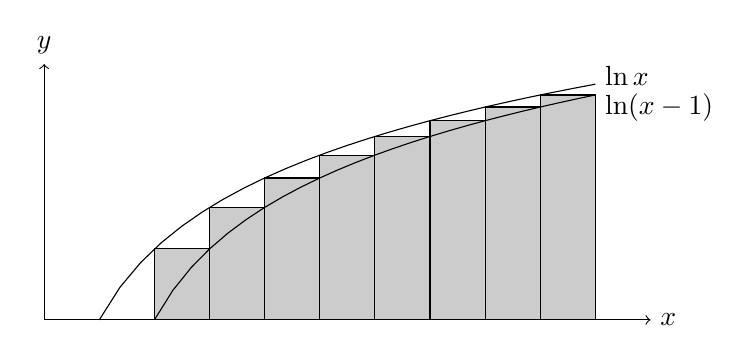
\begin{tikzpicture}[xscale=0.7, yscale=1.3]
     \draw [->] (0, 0) -- (11, 0) node [right] {$x$};
     \draw [->] (0, 0) -- (0, 2.5) node [above] {$y$};
     \draw [domain=2:10] plot (\x, {ln (\x - 1)}) node [anchor = south west] {$\ln x$};
     \draw [domain=1:10] plot (\x, {ln \x }) node [anchor = north west] {$\ln (x - 1)$};
     \draw [fill = black, fill opacity=0.2] (2, 0)-- (2, 0.693147180559945) -- (3, 0.693147180559945) -- (3, 0);
     \draw [fill = black, fill opacity=0.2] (3, 0)-- (3, 1.09861228866811) -- (4, 1.09861228866811) -- (4, 0);
     \draw [fill = black, fill opacity=0.2] (4, 0)-- (4, 1.38629436111989) -- (5, 1.38629436111989) -- (5, 0);
     \draw [fill = black, fill opacity=0.2] (5, 0)-- (5, 1.6094379124341) -- (6, 1.6094379124341) -- (6, 0);
     \draw [fill = black, fill opacity=0.2] (6, 0)-- (6, 1.79175946922806) -- (7, 1.79175946922806) -- (7, 0);
     \draw [fill = black, fill opacity=0.2] (7, 0)-- (7, 1.94591014905531) -- (8, 1.94591014905531) -- (8, 0);
     \draw [fill = black, fill opacity=0.2] (8, 0)-- (8, 2.07944154167984) -- (9, 2.07944154167984) -- (9, 0);
     \draw [fill = black, fill opacity=0.2] (9, 0)-- (9, 2.19722457733622) -- (10, 2.19722457733622) -- (10, 0);
    \end{tikzpicture}
  \end{center}
  Evaluating the integrals gives
  \[
    n\log n - n + 1 \leq \log n! \leq (n+ 1)\log (n + 1) - n.
  \]
  Dividing by $n\log n$ and letting $n\to \infty$, both sides tend to $1$, so
  \[
    \frac{\log n!}{n\log n} \to 1.\qedhere
  \]
\end{proof}

\begin{thm}[Stirling's formula]
  As $n\to \infty$,
  \[
    \log\left(\frac{n!\, e^n}{n^{n + 1/2}}\right) = \log \sqrt{2\pi} + O\left(\frac{1}{n}\right).
  \]
\end{thm}

\begin{cor}
  $n!\sim \sqrt{2\pi}\, n^{n + 1/2}\, e^{-n}$ as $n \to \infty$.
\end{cor}

\begin{proof}[Proof of Stirling's formula (non-examinable)]
  Define the sequence
  \[
    d_n = \log \left(\frac{n!\,e^n}{n^{n + 1/2}}\right) = \log n! - \left(n + \tfrac{1}{2}\right)\log n + n.
  \]
  Then
  \[
    d_n - d_{n + 1} = \left(n + \tfrac{1}{2}\right)\log\left(\frac{n + 1}{n}\right) - 1.
  \]
  Writing $t = 1/(2n + 1)$, so that $(n+1)/n = (1+t)/(1-t)$, this becomes
  \[
    d_n - d_{n + 1} = \frac{1}{2t}\log\left(\frac{1 + t}{1 - t}\right) - 1.
  \]
  Using the Taylor expansions
  \begin{align*}
    \log (1 + t) &= t -\frac{1}{2}t^2 + \frac{1}{3}t^3 - \frac{1}{4}t^4 + \cdots,\\
    \log (1 - t) &= -t -\frac{1}{2}t^2 - \frac{1}{3}t^3 - \frac{1}{4}t^4 - \cdots,
  \end{align*}
  and subtracting, we obtain $\log\bigl(\frac{1+t}{1-t}\bigr) = 2t + \frac{2}{3}t^3 + \frac{2}{5}t^5 + \cdots$. Dividing by $2t$ and subtracting $1$ gives
  \begin{align*}
    d_n - d_{n + 1} &= \frac{1}{3}t^2 + \frac{1}{5}t^4 + \frac{1}{7}t^6 + \cdots\\
    &< \frac{1}{3}t^2 + \frac{1}{3}t^4 + \frac{1}{3}t^6 + \cdots\\
    &= \frac{t^2}{3(1 - t^2)}\\
    &= \frac{1}{3\bigl((2n + 1)^2 - 1\bigr)}\\
    &= \frac{1}{12}\left(\frac{1}{n} - \frac{1}{n + 1}\right).
  \end{align*}
  In particular, $d_n - d_{n+1} > 0$, so $(d_n)$ is strictly decreasing. Summing the bound telescopically,
  \[
    d_n - d_m < \frac{1}{12}\left(\frac{1}{n} - \frac{1}{m}\right) \quad \text{for all } m > n.
  \]
  Setting $n = 1$ shows $d_m > d_1 - \frac{1}{12}$ for all $m$, so $(d_n)$ is bounded below. Being decreasing and bounded below, it converges to a limit $A$. Letting $m \to \infty$ in the bound above gives
  \[
    A \leq d_n < A + \frac{1}{12n}.
  \]

  It remains to identify $A$. Define $I_n = \int_0^{\pi/2} \sin^n\theta\;\d \theta$. Since $0 \leq \sin\theta \leq 1$ on $[0, \pi/2]$, the sequence $(I_n)$ is decreasing. Integration by parts gives the recurrence
  \begin{align*}
    I_n &= \int_0^{\pi/2}\sin^n \theta\;\d \theta = \left[-\cos\theta\sin^{n - 1}\theta \right]_0^{\pi/2} + (n - 1)\int_0^{\pi/2}\cos^2\theta \sin^{n - 2}\theta \;\d\theta\\
    &= (n - 1)(I_{n - 2} - I_n),
  \end{align*}
  so $I_n = \frac{n - 1}{n}\,I_{n - 2}$. Since $I_0 = \pi/2$ and $I_1 = 1$, iterating gives
  \begin{align*}
    I_{2n} &= \frac{1}{2}\cdot\frac{3}{4}\cdots \frac{2n - 1}{2n}\cdot \frac{\pi}{2} = \frac{(2n)!}{(2^n n!)^2}\cdot\frac{\pi}{2},\\
    I_{2n + 1} &= \frac{2}{3}\cdot\frac{4}{5}\cdots\frac{2n}{2n + 1} = \frac{(2^n n!)^2}{(2n + 1)!}.
  \end{align*}
  Since $(I_n)$ is decreasing, $I_{2n+1} \leq I_{2n} \leq I_{2n-1}$, and so
  \[
    1 \leq \frac{I_{2n}}{I_{2n + 1}} \leq \frac{I_{2n - 1}}{I_{2n + 1}} = \frac{2n+1}{2n} \to 1.
  \]
  Using $n!\sim n^{n + 1/2}e^{-n + A}$, we can compute
  \[
    \frac{I_{2n}}{I_{2n + 1}} = \pi(2n + 1)\cdot\frac{\bigl((2n)!\bigr)^2}{2^{4n + 1}(n!)^4} \sim \frac{2\pi}{e^{2A}}.
  \]
  Since $I_{2n}/I_{2n+1} \to 1$, we conclude $e^{2A} = 2\pi$, i.e.\ $A = \log\sqrt{2\pi}$.
\end{proof}

\begin{prop}[Sharper bounds (non-examinable)]
  For all $n \geq 1$,
  \[
    \sqrt{2\pi}\, n^{n + 1/2}\, e^{-n + \frac{1}{12n + 1}} \leq n! \leq \sqrt{2\pi}\, n^{n + 1/2}\, e^{-n + \frac{1}{12n}}.
  \]
\end{prop}

\begin{eg}[Fair coin]
  Suppose a fair coin is tossed $2n$ times. The probability of obtaining exactly $n$ heads and $n$ tails is
  \[
    \frac{\binom{2n}{n}}{2^{2n}} = \frac{(2n)!}{(n!)^2\, 2^{2n}} \sim \frac{1}{\sqrt{n\pi}},
  \]
  by Stirling's formula.
\end{eg}

\begin{eg}[Drawing cards]
  Suppose we draw 26 cards from a standard deck of 52. The probability of obtaining exactly 13 red and 13 black cards is
  \[
    \frac{\binom{26}{13}^2}{\binom{52}{26}} \approx 0.2181.
  \]
\end{eg}
\section{Axioms of probability}
\label{sec:axioms}
\subsection{Axioms and definitions}

\begin{remark}
  In Chapter~1, we defined probability only for finite sample spaces with equally likely outcomes. This is too restrictive for many applications --- for instance, it cannot model a biased coin with $\P(\text{heads}) = \pi^{-1}$. We now give a general axiomatic framework.
\end{remark}

\begin{defi}[Probability space]
  A \emph{probability space} is a triple $(\Omega, \mathcal{F}, \P)$, where:
  \begin{itemize}
    \item $\Omega$ is a set called the \emph{sample space}. Elements of $\Omega$ are called \emph{outcomes}.
    \item $\mathcal{F}$ is a collection of subsets of $\Omega$ satisfying:
    \begin{enumerate}
      \item $\emptyset, \Omega\in \mathcal{F}$;
      \item if $A\in \mathcal{F}$, then $A^C\in \mathcal{F}$;
      \item if $A_1, A_2, \dotsc \in \mathcal{F}$, then $\bigcup_{i = 1}^\infty A_i \in \mathcal{F}$.
    \end{enumerate}
    Elements of $\mathcal{F}$ are called \emph{events}.
    \item $\P\colon \mathcal{F}\to [0, 1]$ is the \emph{probability measure}, satisfying the \emph{Kolmogorov axioms}:
    \begin{enumerate}
      \item $0 \leq \P(A) \leq 1$ for all $A\in \mathcal{F}$;
      \item $\P(\Omega) = 1$;
      \item (\emph{countable additivity}) for any countable collection of pairwise disjoint events $A_1, A_2, \dotsc \in \mathcal{F}$ (i.e.\ $A_i\cap A_j = \emptyset$ for all $i \neq j$),
      \[
        \P\left(\bigcup_{i=1}^{\infty} A_i\right) = \sum_{i=1}^{\infty} \P(A_i).
      \]
    \end{enumerate}
  \end{itemize}
  For an event $A \in \mathcal{F}$, the number $\P(A)$ is called the \emph{probability} of $A$.
\end{defi}

\begin{remark}
  If $\Omega$ is finite or countable, we usually take $\mathcal{F}$ to be the power set of $\Omega$ (i.e.\ the collection of all subsets). If $\Omega$ is uncountable (e.g.\ $\Omega = \R$), one must restrict $\mathcal{F}$ to a suitable collection of subsets in order for $\P$ to be well-defined.
\end{remark}

\begin{defi}[Probability distribution]
  Let $\Omega = \{\omega_1, \omega_2, \dotsc\}$ be a countable sample space. A \emph{probability distribution} on $\Omega$ is a sequence of non-negative numbers $p_1, p_2, \dotsc$ with $\sum_{i = 1}^\infty p_i = 1$. Setting $p(\omega_i) = p_i$, we define
  \[
    \P(A) = \sum_{\omega_i\in A} p(\omega_i)
  \]
  for every event $A \subseteq \Omega$. This defines a probability measure on $\Omega$.
\end{defi}

\begin{prop}[Elementary properties]\leavevmode
  \begin{enumerate}
    \item $\P(\emptyset) = 0$.
    \item $\P(A^C) = 1 - \P(A)$ for any event $A$.
    \item If $A\subseteq B$, then $\P(A) \leq \P(B)$ (monotonicity).
    \item $\P (A\cup B) = \P(A) + \P(B) - \P(A\cap B)$ (inclusion-exclusion for two events).
  \end{enumerate}
\end{prop}

\begin{proof}\leavevmode
  \begin{enumerate}
    \item $\Omega$ and $\emptyset$ are disjoint, so $\P(\Omega) = \P(\Omega \cup \emptyset) = \P(\Omega) + \P(\emptyset)$. Hence $\P(\emptyset) = 0$.
    \item $A$ and $A^C$ are disjoint with $A \cup A^C = \Omega$, so $\P(A) + \P(A^C) = \P(\Omega) = 1$.
    \item Write $B = A\cup (B\cap A^C)$, a disjoint union. Then $\P(B) = \P(A) + \P(B\cap A^C) \geq \P(A)$.
    \item Write $A\cup B = A\cup (B\cap A^C)$, a disjoint union, so $\P(A\cup B) = \P(A) + \P(B\cap A^C)$. Also $B = (A\cap B) \cup (B\cap A^C)$ is a disjoint union, so $\P(B\cap A^C) = \P(B) - \P(A\cap B)$. Substituting gives the result.\qedhere
  \end{enumerate}
\end{proof}

\begin{remark}
  Part (4) implies $\P(A\cup B) \leq \P(A) + \P(B)$, i.e.\ $\P$ is \emph{subadditive}. We also have $\P(A\cap B) + \P(A \cup B) = \P(A) + \P(B)$, so $\P$ is \emph{submodular} (since in general submodularity requires only the inequality $\leq$).
\end{remark}

\begin{defi}[Limit of events]
  Let $A_1, A_2, \dotsc$ be a sequence of events. If the sequence is \emph{increasing}, i.e.\ $A_1 \subseteq A_2 \subseteq \cdots$, we define
  \[
    \lim_{n\to \infty} A_n = \bigcup_{n=1}^\infty A_n.
  \]
  If it is \emph{decreasing}, i.e.\ $A_1\supseteq A_2 \supseteq \cdots$, we define
  \[
    \lim_{n\to \infty} A_n = \bigcap_{n=1}^\infty A_n.
  \]
\end{defi}

\begin{thm}[Continuity of probability]
  Let $A_1, A_2, \dotsc$ be an increasing or decreasing sequence of events. Then
  \[
    \P\left(\lim_{n\to \infty} A_n\right) = \lim_{n\to \infty} \P(A_n).
  \]
\end{thm}

\begin{proof}
  We prove the increasing case. Define $B_1 = A_1$ and $B_n = A_n \setminus A_{n-1}$ for $n \geq 2$. Then $B_1, B_2, \dotsc$ are pairwise disjoint, and
  \[
    \bigcup_{i=1}^n B_i = A_n, \quad \bigcup_{i=1}^\infty B_i = \bigcup_{i=1}^\infty A_i.
  \]
  Therefore
  \begin{align*}
    \P\left(\lim_{n \to \infty} A_n\right) &= \P\left(\bigcup_{i=1}^\infty B_i\right) = \sum_{i=1}^\infty \P(B_i) = \lim_{n \to \infty}\sum_{i = 1}^n \P(B_i) = \lim_{n \to \infty} \P(A_n).
  \end{align*}
  The decreasing case follows by applying the above to the increasing sequence $A_1^C \subseteq A_2^C \subseteq \cdots$ and using $\P(A_n^C) = 1 - \P(A_n)$.
\end{proof}

\subsection{Inequalities and formulae}

\begin{thm}[Boole's inequality / union bound]
  For any events $A_1, A_2, \dotsc$ in a probability space,
  \[
    \P\left(\bigcup_{i = 1}^\infty A_i\right) \leq \sum_{i = 1}^\infty \P(A_i).
  \]
\end{thm}

\begin{proof}
  Define $B_1 = A_1$ and $B_i = A_i\setminus \bigcup_{k = 1}^{i - 1}A_k$ for $i \geq 2$. Then the $B_i$ are pairwise disjoint and $\bigcup_i B_i = \bigcup_i A_i$. Since $B_i \subseteq A_i$, monotonicity gives $\P(B_i) \leq \P(A_i)$. By countable additivity,
  \[
    \P\left(\bigcup_i A_i\right) = \P\left(\bigcup _i B_i\right) = \sum_i \P(B_i) \leq \sum_i \P(A_i).\qedhere
  \]
\end{proof}

\begin{eg}[Infinitely many heads]
  Suppose we toss a countably infinite sequence of biased coins. Let $A_k$ be the event that the $k$th toss is heads, and let $\P(A_k) = p_k$, where $\sum_{k=1}^\infty p_k < \infty$. The event that infinitely many heads occur is
  \[
    \bigcap_{i = 1}^\infty\bigcup_{k = i}^\infty A_k,
  \]
  since this is the event that, for every $i$, at least one head occurs among tosses $i, i+1, i+2, \dotsc$. The sets $C_i = \bigcup_{k=i}^{\infty} A_k$ form a decreasing sequence, so by continuity of $\P$ and Boole's inequality,
  \[
    \P\left(\bigcap_{i = 1}^\infty\bigcup _{k = i}^\infty A_k\right) = \lim_{i \to \infty} \P\left(\bigcup_{k = i}^\infty A_k\right) \leq \lim_{i\to \infty}\sum_{k = i}^\infty p_k = 0.
  \]
  Therefore the probability of infinitely many heads is $0$.
\end{eg}

\begin{eg}[Erd\H{o}s 1947 --- Ramsey lower bound]
  Let $n, k \geq 1$ be integers. Consider the complete graph $K_n$ on $n$ vertices (i.e.\ the graph with an edge between every pair of vertices). We ask: is it possible to $2$-colour the edges of $K_n$ (say red and blue) so that no complete subgraph on $k$ vertices is monochromatic?

  Colour each edge independently and uniformly at random. For each $k$-element subset $S$ of vertices, let $A_S$ be the event that all $\binom{k}{2}$ edges of $S$ receive the same colour. Then $\P(A_S) = 2 \cdot 2^{-\binom{k}{2}}$, since the subgraph can be monochromatic in either colour. By Boole's inequality,
  \[
    \P\left(\bigcup_S A_S\right) \leq \sum_S \P(A_S) = \binom{n}{k}\cdot 2^{1 - \binom{k}{2}}.
  \]
  If $\binom{n}{k}\, 2^{1 - \binom{k}{2}} < 1$, then this probability is strictly less than $1$, so there exists a colouring with no monochromatic $k$-clique.
\end{eg}

\begin{thm}[Inclusion-exclusion formula]
  Let $A_1, A_2, \dotsc, A_n$ be events. Then
  \begin{align*}
    \P\left(\bigcup_{i=1}^n A_i\right) &= \sum_{i} \P(A_i) - \sum_{i_1 < i_2} \P(A_{i_1}\cap A_{i_2}) + \sum_{i_1 < i_2 < i_3}\P(A_{i_1}\cap A_{i_2} \cap A_{i_3}) - \cdots\\
    &\quad + (-1)^{n - 1} \P(A_1\cap \cdots \cap A_n).
  \end{align*}
\end{thm}

\begin{proof}
  By induction on $n$. The case $n = 2$ is the inclusion-exclusion identity for two events. For the inductive step, write
  \[
    \P\left(\bigcup_{i=1}^{n} A_i\right) = \P(A_1) + \P\left(\bigcup_{i = 2}^n A_i\right) - \P\left(\bigcup_{i = 2}^n (A_1\cap A_i)\right)
  \]
  and apply the inductive hypothesis to the two unions of $n-1$ events on the right-hand side.
\end{proof}

\begin{eg}[Derangements]
  Let $\pi$ be a uniformly random permutation of $\{1, 2, \dotsc, n\}$. A \emph{derangement} is a permutation with no fixed points, i.e.\ $\pi(i) \neq i$ for all $i$. Let $A_i = \{\pi(i) = i\}$ be the event that $i$ is a fixed point.

  By symmetry, for any subset $\{i_1, \dotsc, i_r\} \subseteq \{1, \dotsc, n\}$,
  \[
    \P(A_{i_1} \cap \cdots \cap A_{i_r}) = \frac{(n-r)!}{n!},
  \]
  since there are $(n-r)!$ permutations fixing all of $i_1, \dotsc, i_r$. Since there are $\binom{n}{r}$ such subsets, inclusion-exclusion gives
  \begin{align*}
    \P\left(\bigcup_{i = 1}^n A_i\right) &= \sum_{r=1}^{n} (-1)^{r-1} \binom{n}{r} \frac{(n-r)!}{n!} = \sum_{r=1}^{n} \frac{(-1)^{r-1}}{r!} \to 1 - e^{-1}.
  \end{align*}
  Therefore, for large $n$, the probability of a derangement is approximately $1 - (1 - e^{-1}) = e^{-1}\approx 0.368$.
\end{eg}

\begin{thm}[Bonferroni's inequalities]
  Let $A_1, A_2, \dotsc, A_n$ be events and let $1 \leq r\leq n$. For $1 \leq j \leq n$, define the $j$th inclusion-exclusion term
  \[
    S_j = \sum_{i_1 < i_2 < \cdots < i_j} \P(A_{i_1}\cap A_{i_2}\cap \cdots \cap A_{i_j}).
  \]
  If $r$ is odd, then
  \[
    \P\left(\bigcup_{i=1}^n A_i\right) \leq S_1 - S_2 + S_3 - \cdots + S_r.
  \]
  If $r$ is even, then
  \[
    \P\left(\bigcup_{i=1}^n A_i\right) \geq S_1 - S_2 + S_3 - \cdots - S_r.
  \]
\end{thm}

\begin{remark}
  The case $r = 1$ recovers Boole's inequality. The case $r = n$ recovers the inclusion-exclusion formula with equality.
\end{remark}

\begin{proof}
  By induction on $n$.
\end{proof}

\begin{eg}[Bonferroni applied to initial segments]
  Let $m \geq 1$ and let $\Omega = \{1, 2, \dotsc, m\}$ with uniform probabilities. For $1 \leq k \leq m$, define $A_k = \{1, 2, \dotsc, k\}$, so that $\P(A_k) = k/m$. Then for any $j, k$,
  \[
    A_j \cap A_k = A_{\min(j, k)}, \qquad A_j \cup A_k = A_{\max(j, k)}.
  \]
  Let $x_1, \dotsc, x_n \in \{1, \dotsc, m\}$. Applying Bonferroni's inequality with $r = 2$ gives
  \[
    \frac{\max\{x_1, \dotsc, x_n\}}{m} = \P\left(\bigcup_{i=1}^{n} A_{x_{i}}\right) \geq \sum_{i=1}^{n} \frac{x_i}{m} - \sum_{i < j} \frac{\min\{x_i, x_j\}}{m},
  \]
  and hence $\max\{x_1, \dotsc, x_n\} \geq \sum_i x_i - \sum_{i < j} \min\{x_i, x_j\}$.
\end{eg}

\subsection{Independence}

\begin{defi}[Independent events]
  Two events $A$ and $B$ are \emph{independent} if
  \[
    \P(A\cap B) = \P(A)\,\P(B).
  \]
  Otherwise, they are said to be \emph{dependent}.
\end{defi}

\begin{prop}
  If $A$ and $B$ are independent, then $A$ and $B^C$ are independent.
\end{prop}

\begin{proof}
  \begin{align*}
    \P(A\cap B^C) &= \P(A) - \P(A\cap B) = \P(A) - \P(A)\,\P(B) = \P(A)\bigl(1 - \P(B)\bigr) = \P(A)\,\P(B^C).\qedhere
  \end{align*}
\end{proof}

\begin{eg}[Pairwise independence does not imply mutual independence]
  Roll two fair dice. Let $A_1$ be the event that the first die is odd, $A_2$ the event that the second die is odd, and $A_3$ the event that the sum is odd. The relevant probabilities are:
  \begin{center}
    \begin{tabular}{cc}
      \toprule
      Event & Probability\\
      \midrule
      $A_1$ & $1/2$\\
      $A_2$ & $1/2$\\
      $A_3$ & $1/2$\\
      $A_1\cap A_2$ & $1/4$\\
      $A_1\cap A_3$ & $1/4$\\
      $A_2\cap A_3$ & $1/4$\\
      $A_1\cap A_2\cap A_3$ & $0$\\
      \bottomrule
    \end{tabular}
  \end{center}
  Every pair is independent (e.g.\ $\P(A_1 \cap A_2) = 1/4 = \P(A_1)\,\P(A_2)$), but the three events are not mutually independent, since $\P(A_1\cap A_2\cap A_3) = 0 \neq 1/8 = \P(A_1)\,\P(A_2)\,\P(A_3)$.
\end{eg}

\begin{defi}[Mutual independence]
  Events $A_1, A_2, \dotsc$ are \emph{mutually independent} if for every finite subset of distinct indices $i_1, i_2, \dotsc, i_r$ with $r \geq 2$,
  \[
    \P(A_{i_1}\cap A_{i_2} \cap \cdots \cap A_{i_r}) = \P(A_{i_1})\,\P(A_{i_2})\cdots \P(A_{i_r}).
  \]
\end{defi}

\begin{eg}[Matching dice]
  Roll 4 fair dice. For $1 \leq i < j \leq 4$, let $A_{ij}$ be the event that dice $i$ and $j$ show the same value. Then $\P(A_{ij}) = 1/6$ for each pair. We have
  \[
    \P(A_{12}\cap A_{13}) = \frac{1}{36} = \P(A_{12})\,\P(A_{13}),
  \]
  since dice 1, 2 and 3 must all show the same value. However,
  \[
    \P(A_{12}\cap A_{13}\cap A_{23}) = \frac{1}{36} \neq \frac{1}{216} = \P(A_{12})\,\P(A_{13})\,\P(A_{23}),
  \]
  since $A_{23}$ is implied by $A_{12} \cap A_{13}$. So these events are not mutually independent.
\end{eg}

\begin{defi}[Product of probability spaces]
  Let $(\Omega_1, \mathcal{F}_1, \P_1)$ and $(\Omega_2, \mathcal{F}_2, \P_2)$ be two probability spaces with $\Omega_1 = \{\alpha_1, \alpha_2, \dotsc\}$ and $\Omega_2 = \{\beta_1, \beta_2, \dotsc\}$. The \emph{product probability space} is $\Omega = \Omega_1\times \Omega_2$ with
  \[
    \P\bigl((\alpha_i, \beta_j)\bigr) = \P_1(\alpha_i)\,\P_2(\beta_j)
  \]
  for all $i, j$.
\end{defi}

\begin{prop}
  In the product space, let $A\subseteq \Omega_1$ and $B\subseteq \Omega_2$ be events. Viewing these as events in $\Omega$ via $A \times \Omega_2$ and $\Omega_1 \times B$ respectively, we have $\P(A\cap B) = \P_1(A)\,\P_2(B)$. That is, events from different component experiments are independent.
\end{prop}

\begin{proof}
  Writing $p_i = \P_1(\alpha_i)$ and $q_j = \P_2(\beta_j)$,
  \[
    \P(A\cap B) = \sum_{\alpha_i\in A}\sum_{\beta_j\in B} p_i\, q_j = \left(\sum_{\alpha_i\in A} p_i\right)\left(\sum_{\beta_j\in B}q_j\right) = \P_1(A)\,\P_2(B).\qedhere
  \]
\end{proof}

\begin{remark}
  This construction generalises to products of $n$ or even countably many probability spaces.
\end{remark}


\subsection{Important discrete distributions}

\begin{defi}[Bernoulli distribution]
  Let $p\in [0, 1]$. A random variable with the \emph{Bernoulli distribution} $B(1, p)$ takes values in $\{0, 1\}$ with
  \[
    \P(X = 1) = p, \qquad \P(X = 0) = 1- p.
  \]
  We think of $1$ as ``success'' and $0$ as ``failure''.
\end{defi}

\begin{defi}[Binomial distribution]
  Let $n \geq 1$ be an integer and $p \in [0,1]$. The \emph{binomial distribution} $B(n, p)$ is the distribution of the number of successes in $n$ independent Bernoulli trials, each with success probability $p$. It takes values in $\{0, 1, \dotsc, n\}$ with
  \[
    \P(X = k) = \binom{n}{k}p^k(1 - p)^{n - k}, \qquad k = 0, 1, \dotsc, n.
  \]
\end{defi}

\begin{defi}[Geometric distribution]
  Let $p \in (0, 1]$. The \emph{geometric distribution} $\mathrm{Geom}(p)$ is the distribution of the number of failures before the first success in a sequence of independent Bernoulli trials with success probability $p$. It takes values in $\{0, 1, 2, \dotsc\}$ with
  \[
    \P(X = k) = (1- p)^k\, p, \qquad k = 0, 1, 2, \dotsc
  \]
\end{defi}

\begin{remark}
  The geometric distribution is \emph{memoryless}: given that no success has occurred in the first $m$ trials, the number of additional trials until the first success has the same distribution as the original. This is because the remaining trials are still independent Bernoulli trials with the same parameter $p$.
\end{remark}

\begin{defi}[Hypergeometric distribution]
  Suppose an urn contains $n_1$ red balls and $n_2$ black balls. We draw $n \leq n_1 + n_2$ balls without replacement. The number of red balls drawn has the \emph{hypergeometric distribution}: for $\max(0, n - n_2) \leq k \leq \min(n, n_1)$,
  \[
    \P(X = k) = \frac{\binom{n_1}{k}\binom{n_2}{n - k}}{\binom{n_1 + n_2}{n}}.
  \]
\end{defi}

\begin{defi}[Poisson distribution]
  Let $\lambda > 0$. The \emph{Poisson distribution} $\mathrm{Poisson}(\lambda)$ takes values in $\{0, 1, 2, \dotsc\}$ with
  \[
    \P(X = k) = \frac{\lambda^k}{k!}\,e^{-\lambda}, \qquad k = 0, 1, 2, \dotsc
  \]
\end{defi}

\begin{remark}
  The Poisson distribution models the number of occurrences of a rare event. Informally, if an event occurs at rate $\lambda$ over many independent trials --- say $n$ trials each with success probability $\lambda/n$ --- then as $n \to \infty$, the number of successes approaches a $\mathrm{Poisson}(\lambda)$ distribution. The following theorem makes this precise.
\end{remark}

\begin{thm}[Poisson approximation to the binomial]
  Let $\lambda > 0$ be fixed, and let $k \geq 0$ be a fixed integer. If $n\to \infty$ and $p = p_n \to 0$ in such a way that $np \to \lambda$, then
  \[
    \binom{n}{k}p^k(1 -p)^{n - k} \to \frac{\lambda^k}{k!}\,e^{-\lambda}.
  \]
\end{thm}

\begin{proof}
  Write $q_k = \binom{n}{k}p^k(1 - p)^{n - k}$. Then
  \begin{align*}
    q_k &= \frac{1}{k!} \cdot \frac{n(n - 1)\cdots(n - k + 1)}{n^k}\cdot (np)^k \cdot \left(1 - \frac{np}{n}\right)^{n - k}.
  \end{align*}
  As $n \to \infty$ with $np \to \lambda$: the ratio $n(n-1)\cdots(n-k+1)/n^k \to 1$ (since $k$ is fixed), $(np)^k \to \lambda^k$, and $(1 - np/n)^{n-k} \to e^{-\lambda}$ (since $(1 - a/n)^n \to e^{-a}$). Hence $q_k \to \lambda^k e^{-\lambda}/k!$.
\end{proof}
\subsection{Conditional probability}

\begin{defi}[Conditional probability]
  Let $B$ be an event with $\P(B) > 0$. For any event $A$, the \emph{conditional probability of $A$ given $B$} is
  \[
    \P(A\mid B) = \frac{\P(A\cap B)}{\P(B)}.
  \]
\end{defi}

\begin{remark}
  If $A$ and $B$ are independent, then $\P(A\mid B) = \P(A)$, since $\P(A \cap B) = \P(A)\,\P(B)$.
\end{remark}

\begin{defi}[Attraction and repulsion]
  We say that $B$ \emph{attracts} $A$ if $\P(A\mid B) > \P(A)$. Since
  \[
    \frac{\P(A\cap B)}{\P(B)} > \P(A) \iff \frac{\P(A\cap B)}{\P(A)} > \P(B),
  \]
  attraction is symmetric: $B$ attracts $A$ if and only if $A$ attracts $B$. We say $B$ \emph{repels} $A$ if $B^C$ attracts $A$.
\end{defi}

\begin{eg}[Poker hands]
  In a game of poker, let $A_i$ be the event that player $i$ is dealt a royal flush. Then $\P(A_1) = 1.539\times 10^{-6}$, while $\P(A_2\mid A_1) = 1.969\times 10^{-6}$. Since $\P(A_2 \mid A_1) > \P(A_2)$, good hands attract: given that player 1 has a royal flush, it is (slightly) more likely that player 2 also has one.
\end{eg}

\begin{prop}[Properties of conditional probability]\leavevmode
  \begin{enumerate}
    \item (Multiplication rule) $\P(A\cap B) = \P(A\mid B)\,\P(B)$.
    \item (Chain rule) $\P(A\cap B\cap C) = \P(A\mid B\cap C)\, \P(B\mid C)\, \P(C)$.
    \item $\P(A\mid B\cap C) = \dfrac{\P(A\cap B\mid C)}{\P(B\mid C)}$, provided $\P(B \cap C) > 0$.
    \item The function $\P(\ph \mid B)$, restricted to subsets of $B$, is a probability measure on $B$.
  \end{enumerate}
\end{prop}

\begin{proof}
  Parts (1)--(3) follow directly from the definition. For (4), we verify the Kolmogorov axioms:
  \begin{enumerate}
    \item For $A\subseteq B$, $\P(A\mid B) = \P(A\cap B)/\P(B) = \P(A)/\P(B) \leq 1$.
    \item $\P(B\mid B) = \P(B)/\P(B) = 1$.
    \item Let $A_1, A_2, \dotsc$ be pairwise disjoint events with $A_i \subseteq B$ for all $i$. Then
      \[
        \P\left(\left.\bigcup_i A_i\right\vert B\right) = \frac{\P\bigl(\bigcup_i A_i\bigr)}{\P(B)} = \sum_i \frac{\P(A_i)}{\P(B)} = \sum_i \P(A_i \mid B).\qedhere
      \]
  \end{enumerate}
\end{proof}

\begin{defi}[Partition]
  A \emph{partition} of the sample space $\Omega$ is a countable collection of pairwise disjoint events $B_1, B_2, \dotsc$ with $\P(B_i) > 0$ for all $i$ and $\bigcup_i B_i = \Omega$.
\end{defi}

\begin{eg}
  When rolling a die, the events ``odd'' $= \{1,3,5\}$ and ``even'' $= \{2,4,6\}$ form a partition of $\Omega = \{1, \dotsc, 6\}$.
\end{eg}

\begin{prop}[Law of total probability]
  Let $B_1, B_2, \dotsc$ be a partition of $\Omega$, and let $A$ be any event. Then
  \[
    \P(A) = \sum_{i} \P(A\cap B_i) = \sum_{i} \P(A\mid B_i)\, \P(B_i).
  \]
\end{prop}

\begin{eg}[Gambler's ruin]
  A gambler starts with $\$x$ and tosses a fair coin repeatedly, winning $\$1$ for heads and losing $\$1$ for tails. The game ends when the gambler is broke or reaches $\$a$, where $a > x > 0$ is a fixed target. Let
  \[
    p_x = \P(\text{goes broke}\mid \text{starts with }\$x).
  \]
  Let $H$ be the event that the first toss is heads. By the law of total probability,
  \[
    p_x = \P(H)\,p_{x + 1} + \P(H^C)\, p_{x - 1} = \frac{1}{2}\,p_{x + 1} + \frac{1}{2}\,p_{x - 1}.
  \]
  With boundary conditions $p_0 = 1$ and $p_a = 0$, solving this recurrence gives $p_x = 1 - x/a$.
\end{eg}

\begin{thm}[Bayes' formula]
  Let $B_1, B_2, \dotsc$ be a partition of $\Omega$, and let $A$ be an event with $\P(A) > 0$. Then for each $i$,
  \[
    \P(B_i \mid A) = \frac{\P(A \mid B_i)\,\P(B_i)}{\sum_j\P(A \mid B_j)\,\P(B_j)}.
  \]
\end{thm}

\begin{remark}
  The denominator is simply $\P(A)$, expressed via the law of total probability. Bayes' formula ``inverts'' the conditioning: given $\P(A \mid B_i)$ and the prior probabilities $\P(B_i)$, it computes the posterior probability $\P(B_i \mid A)$.
\end{remark}

\begin{eg}[Screening test]
  A screening test for a disease has the following characteristics: let $D$ be the event that a patient has the disease and $+$ the event of a positive test result. Suppose
  \[
    \P(+ \mid D) = 0.98, \qquad \P(+ \mid D^C) = 0.01, \qquad \P(D) = 0.001.
  \]
  By Bayes' formula,
  \begin{align*}
    \P(D\mid +) &= \frac{\P(+ \mid D)\,\P(D)}{\P(+\mid D)\,\P(D) + \P(+\mid D^C)\,\P(D^C)} = \frac{0.98\cdot 0.001}{0.98\cdot 0.001 + 0.01\cdot 0.999} \approx 0.09.
  \end{align*}
  Despite the test's high sensitivity, the low prevalence of the disease means that a positive result is far more likely to be a false positive than a true positive.
\end{eg}

\begin{eg}[Boy born on a Tuesday]
  Suppose a family has two children, each equally likely to be a boy or a girl, independently. Consider two scenarios:
  \begin{enumerate}
    \item Given that at least one child is a boy, the probability that both are boys is
    \[
      \P(BB\mid \text{at least one }B) = \frac{\P(BB)}{\P(BB) + \P(BG) + \P(GB)} = \frac{1/4}{3/4} = \frac{1}{3}.
    \]
    \item Now suppose each child is equally likely to be born on any of 7 days. Given that at least one child is a boy born on a Tuesday, the probability that both are boys is $13/27$.
  \end{enumerate}
  To see (2), let $B^*$ denote a boy born on a Tuesday (probability $1/14$ per child) and let $C$ be the event that at least one child is $B^*$. Each child is one of $14$ equally likely types ($2$ sexes $\times$ $7$ days), so the pair has $14^2 = 196$ equally likely outcomes. The number of outcomes in which at least one child is $B^*$ is $2 \cdot 14 - 1 = 27$ (by inclusion-exclusion). Among these, the number in which both children are boys is $2 \cdot 7 - 1 = 13$ (both are boys, at least one born on Tuesday). Hence $\P(\text{both boys} \mid C) = 13/27$.

  The shift from $1/3$ to $13/27 \approx 0.481$ occurs because having two boys makes it more likely that at least one is born on a specific day, so the extra information shifts the posterior toward two boys.
\end{eg}

\section{Discrete random variables}
With what we've got so far, we are able to answer questions like ``what is the probability of getting a heads?'' or ``what is the probability of getting 10 heads in a row?''. However, we cannot answer questions like ``what do we expect to get on average?''. What does it even mean to take the average of a ``heads'' and a ``tail''?

To make some sense of this notion, we have to assign, to each outcome, a number. For example, if let ``heads'' correspond to $1$ and ``tails'' correspond to $0$. Then on average, we can expect to get $0.5$. This is the idea of a random variable.

\subsection{Discrete random variables}

\begin{defi}[Random variable]
  A \emph{random variable} $X$ is a function $X\colon \Omega \to \Omega_X$, where $\Omega_X$ is a set (usually $\R$ or a subset of $\R$). A random variable is \emph{discrete} if $\Omega_X$ is finite or countably infinite.
\end{defi}

\begin{notation}
  For $T\subseteq \Omega_X$, we write
  \[
    \P(X\in T) = \P(\{\omega \in \Omega: X(\omega) \in T\}).
  \]
  We write $\P_X(x) = \P(X = x)$ for the \emph{probability mass function} of $X$. If $X$ has a named distribution, we write e.g.\ $X\sim B(n, p)$ to mean $\P(X = k) = \binom{n}{k}p^k(1 - p)^{n - k}$ for $k = 0, 1, \dotsc, n$.
\end{notation}

\begin{defi}[Discrete uniform distribution]
  A discrete random variable has the \emph{discrete uniform distribution} on a finite set $S$ if $\P(X = s) = 1/|S|$ for all $s \in S$.
\end{defi}

\begin{eg}
  Let $X$ be the value shown by rolling a fair die. Then $X$ has the discrete uniform distribution on $\{1, 2, 3, 4, 5, 6\}$, with $\P(X = i) = 1/6$ for each $i$.
\end{eg}

\begin{eg}[Sum of two dice]
  If $X$ and $Y$ are the values of two independent fair dice, then $X + Y$ is a new random variable taking values in $\{2, 3, \dotsc, 12\}$.
\end{eg}

\begin{defi}[Expectation]
  The \emph{expectation} (or \emph{mean}) of a discrete real-valued random variable $X$ is
  \[
    \E[X] = \sum_{x\in \Omega_X}x\,\P(X = x),
  \]
  provided this sum is absolutely convergent. Equivalently, $\E[X] = \sum_{\omega\in \Omega}p_\omega\, X(\omega)$, where $p_\omega = \P(\{\omega\})$.
\end{defi}

\begin{eg}[Sum of two dice]
  Let $X$ be the sum of the outcomes of two fair dice. Then
  \[
    \E[X] = 2\cdot \frac{1}{36} + 3\cdot \frac{2}{36} + \cdots + 12\cdot \frac{1}{36} = 7.
  \]
\end{eg}

\begin{eg}[St.\ Petersburg paradox]
  A fair coin is tossed repeatedly until the first tail appears. If the first tail occurs on toss $i$, the player receives $\$2^i$. The expected payout is
  \[
    \E[X] = \sum_{i=1}^{\infty} 2^i \cdot \frac{1}{2^i} = \sum_{i=1}^{\infty} 1 = \infty.
  \]
  The expected value is infinite, yet few people would pay more than $\$20$ to play. This illustrates that expected value alone does not capture rational decision-making under uncertainty.
\end{eg}

\begin{eg}[Expectation of the Poisson distribution]
  Let $X\sim \mathrm{Poisson}(\lambda)$. Then
  \begin{align*}
    \E[X] &= \sum_{r = 0}^\infty r\,\frac{\lambda^r e^{-\lambda}}{r!} = \sum_{r = 1}^\infty \lambda\, \frac{\lambda^{r - 1}e^{-\lambda}}{(r - 1)!} = \lambda\sum_{r = 0}^\infty\frac{\lambda^r e^{-\lambda}}{r!} = \lambda.
  \end{align*}
\end{eg}

\begin{eg}[Expectation of the binomial distribution]
  Let $X\sim B(n, p)$. Then
  \begin{align*}
    \E[X] &= \sum_{r=0}^n r\binom{n}{r} p^r(1 - p)^{n - r} = np\sum_{r = 1}^n \binom{n - 1}{r-1}p^{r - 1}(1 - p)^{n - 1 - (r - 1)} = np,
  \end{align*}
  since the remaining sum equals $(p + (1-p))^{n-1} = 1$.
\end{eg}

\begin{defi}[Functions of a random variable]
  Let $X$ be a random variable and $f\colon \R \to \R$. Then $f(X)$ is the random variable defined by $f(X)(\omega) = f(X(\omega))$.
\end{defi}

\begin{prop}[Properties of expectation]\leavevmode
  \begin{enumerate}
    \item If $X \geq 0$, then $\E[X] \geq 0$.
    \item If $X\geq 0$ and $\E[X] = 0$, then $\P(X = 0) = 1$.
    \item (Linearity) For constants $a, b \in \R$, $\E[a + bX] = a + b\,\E[X]$.
    \item (Additivity) For any random variables $X$ and $Y$, $\E[X + Y] = \E[X] + \E[Y]$, regardless of whether $X$ and $Y$ are independent.
    \item The constant $c$ that minimises $\E[(X - c)^2]$ is $c = \E[X]$.
  \end{enumerate}
\end{prop}

\begin{proof}\leavevmode
  \begin{enumerate}
    \item $\E[X] = \sum_\omega p_\omega X(\omega) \geq 0$ since every term is non-negative.
    \item If $X(\omega) > 0$ for some $\omega$ with $p_\omega > 0$, then $\E[X] > 0$. Hence $\P(X = 0) = 1$.
    \item $\E[a + bX] = \sum_\omega (a + bX(\omega))\,p_\omega = a\sum_\omega p_\omega + b\sum_\omega X(\omega)\,p_\omega = a + b\,\E[X]$.
    \item $\E[X + Y] = \sum_\omega p_\omega(X(\omega) + Y(\omega)) = \E[X] + \E[Y]$.
    \item Write $\E[(X - c)^2] = \E[(X - \E[X])^2] + (\E[X] - c)^2$, using $\E[X - \E[X]] = 0$ to eliminate the cross term. This is minimised when $c = \E[X]$.\qedhere
  \end{enumerate}
\end{proof}

\begin{prop}[Linearity of expectation for finite sums]
  For any random variables $X_1, \dotsc, X_n$ whose expectations exist,
  \[
    \E\left[\sum_{i = 1}^n X_i\right] = \sum_{i = 1}^n \E[X_i].
  \]
\end{prop}

\begin{proof}
  Immediate from additivity and induction on $n$.
\end{proof}

\begin{defi}[Variance and standard deviation]
  The \emph{variance} of a random variable $X$ with finite expectation is
  \[
    \var(X) = \E[(X - \E[X])^2].
  \]
  The \emph{standard deviation} of $X$ is $\sqrt{\var(X)}$. The variance measures how dispersed $X$ is around its mean.
\end{defi}

\begin{prop}[Properties of variance]\leavevmode
  \begin{enumerate}
    \item $\var(X) \geq 0$, with equality if and only if $\P(X = \E[X]) = 1$.
    \item For constants $a, b \in \R$, $\var(a + bX) = b^2\, \var(X)$.
    \item $\var(X) = \E[X^2] - (\E[X])^2$.
  \end{enumerate}
\end{prop}

\begin{proof}
  Part (1) follows from the fact that $(X - \E[X])^2 \geq 0$. Parts (2) and (3) follow by expanding the definition and using linearity of expectation.
\end{proof}

\begin{eg}[Variance of the binomial distribution]
  Let $X\sim B(n, p)$ and write $q = 1 - p$. Using the factorial moment,
  \begin{align*}
    \E[X(X - 1)] &= \sum_{r = 0}^n r(r - 1)\binom{n}{r} p^r q^{n - r} = n(n - 1)p^2\sum_{r = 2}^n \binom{n - 2}{r - 2} p^{r - 2}q^{n - 2 - (r - 2)} = n(n - 1)p^2,
  \end{align*}
  so $\E[X^2] = n(n - 1)p^2 + np$ and $\var(X) = \E[X^2] - (np)^2 = np(1 - p) = npq$.
\end{eg}

\begin{eg}[Variance of the Poisson distribution]
  Let $X\sim \mathrm{Poisson}(\lambda)$. A similar factorial moment computation gives $\E[X(X-1)] = \lambda^2$, so $\E[X^2] = \lambda^2 + \lambda$ and $\var(X) = \lambda$.
\end{eg}

\begin{eg}[Variance of the geometric distribution]
  Let $X\sim \mathrm{Geom}(p)$, so $\P(X = r) = q^r p$ for $r= 0, 1, 2, \dotsc$, where $q = 1 - p$. Using the generating function $\sum_{r=0}^{\infty} q^r = (1 - q)^{-1}$ and differentiating,
  \begin{align*}
    \E[X] &= pq\sum_{r=0}^\infty rq^{r - 1} = pq\,\frac{\d }{\d q}\frac{1}{1 - q} = \frac{pq}{(1 - q)^2} = \frac{q}{p}.
  \end{align*}
  Similarly, $\E[X(X - 1)] = 2q^2/p^2$, and so $\var(X) = \E[X(X-1)] + \E[X] - (\E[X])^2 = q/p^2$.
\end{eg}

\begin{defi}[Indicator function]
  The \emph{indicator function} (or \emph{indicator variable}) of an event $A\subseteq \Omega$ is the random variable
  \[
    I_A(\omega) =
    \begin{cases}
      1 & \text{if } \omega\in A,\\
      0 & \text{if } \omega\not\in A.
    \end{cases}
  \]
\end{defi}

\begin{prop}[Properties of indicator functions]
  Let $A, B \subseteq \Omega$ be events. Then:
  \begin{enumerate}
    \item $\E[I_A] = \P(A)$.
    \item $I_{A^C} = 1 - I_A$.
    \item $I_{A\cap B} = I_A\, I_B$.
    \item $I_{A\cup B} = I_A + I_B - I_A\, I_B$.
    \item $I_A^2 = I_A$.
  \end{enumerate}
\end{prop}

\begin{proof}
  Each identity follows from the fact that $I_A(\omega) \in \{0, 1\}$ and by checking both cases.
\end{proof}

\begin{eg}[Couples at a dinner table]
  Let $2n$ people ($n$ married couples, $n > 2$) sit in alternating man-woman positions around a circular table, uniformly at random. Let $N$ be the number of couples sitting next to each other, and let $A_i$ be the event that the $i$th couple sits together. Then $N = \sum_{i = 1}^n I_{A_i}$.

  By symmetry, $\P(A_i) = 2/n$ for each $i$ (each wife has $n$ possible seats, and 2 of them are adjacent to her husband). So
  \[
    \E[N] = \sum_{i=1}^n \P(A_i) = n\cdot \frac{2}{n} = 2.
  \]
  To find $\var(N)$, we compute $\E[N^2] = \sum_i \E[I_{A_i}] + 2\sum_{i < j}\P(A_i \cap A_j)$.  One finds $\P(A_1\cap A_2) = \frac{2}{n}\bigl(\frac{1}{(n - 1)^2} + \frac{2(n - 2)}{(n - 1)^2}\bigr)$, which gives $\var(N) = \frac{2(n- 2)}{n - 1}$.

  In fact, as $n\to \infty$, $N$ converges in distribution to $\mathrm{Poisson}(2)$.
\end{eg}

\begin{thm}[Inclusion-exclusion via indicators]
  Let $A_1, \dotsc, A_n$ be events. Then
  \begin{align*}
    \P\left(\bigcup_{i=1}^n A_i\right) &= \sum_{i} \P(A_i) - \sum_{i_1 < i_2} \P(A_{i_1}\cap A_{i_2}) + \cdots + (-1)^{n - 1} \P(A_1\cap \cdots \cap A_n).
  \end{align*}
\end{thm}

\begin{proof}
  Let $I_j = I_{A_j}$. For $1 \leq r \leq n$, define $S_r = \sum_{i_1 < \cdots < i_r}I_{i_1}\cdots I_{i_r}$ and $s_r = \E[S_r] = \sum_{i_1 < \cdots < i_r}\P(A_{i_1}\cap \cdots \cap A_{i_r})$. Expanding the product gives the identity
  \[
    I_{\bigcup_j A_j} = 1 - \prod_{j = 1}^n(1 - I_j) = S_1 - S_2 + S_3 - \cdots + (-1)^{n - 1}S_n.
  \]
  Taking expectations yields $\P\bigl(\bigcup_j A_j\bigr) = s_1 - s_2 + s_3 - \cdots + (-1)^{n - 1}s_n$.
\end{proof}

\begin{defi}[Independent random variables]
  Discrete random variables $X_1, X_2, \dotsc, X_n$ are \emph{independent} if for all $x_1, x_2, \dotsc, x_n$,
  \[
    \P(X_1 = x_1, \dotsc, X_n = x_n) = \P(X_1 = x_1)\cdots \P(X_n = x_n).
  \]
\end{defi}

\begin{prop}
  If $X_1, \dotsc, X_n$ are independent random variables and $f_1, \dotsc, f_n\colon \R \to \R$, then $f_1(X_1), \dotsc, f_n(X_n)$ are independent.
\end{prop}

\begin{proof}
  For any $y_1, \dotsc, y_n$,
  \begin{align*}
    \P(f_1(X_1) = y_1, \dotsc, f_n(X_n) = y_n) &= \sum_{\substack{x_1: f_1(x_1) = y_1\\\vdots\\x_n: f_n(x_n) = y_n}} \prod_{i = 1}^n \P(X_i = x_i) = \prod_{i = 1}^n \sum_{x_i:f_i(x_i) = y_i} \P(X_i = x_i) = \prod_{i = 1}^n \P(f_i(X_i) = y_i),
  \end{align*}
  where the factorisation of the multi-sum into a product of single sums holds because the summand is a product of terms each depending on a single index.
\end{proof}

\begin{thm}[Expectation of a product of independent random variables]
  If $X_1, \dotsc, X_n$ are independent random variables with finite expectations, then
  \[
    \E\left[\prod_{i=1}^{n} X_i\right] = \prod_{i=1}^{n} \E[X_i].
  \]
\end{thm}

\begin{proof}
  Let $R_i$ denote the range of $X_i$. Then
  \begin{align*}
    \E\left[\prod_{i=1}^n X_i\right] &= \sum_{x_1\in R_1}\cdots \sum_{x_n\in R_n}\left(\prod_{i=1}^{n} x_i\right) \P(X_1 = x_1, \dotsc, X_n = x_n)\\
    &= \prod_{i = 1}^n \sum_{x_i \in R_i}x_i\,\P(X_i = x_i) = \prod_{i = 1}^n \E[X_i].\qedhere
  \end{align*}
\end{proof}

\begin{cor}
  If $X_1,\dotsc, X_n$ are independent and $f_1, \dotsc, f_n\colon \R\to \R$, then
  \[
    \E\left[\prod_{i=1}^{n} f_i(X_i)\right] = \prod_{i=1}^{n} \E[f_i(X_i)].
  \]
\end{cor}

\begin{thm}[Variance of a sum of independent random variables]
  If $X_1, X_2, \dotsc, X_n$ are independent random variables with finite variances, then
  \[
    \var\left(\sum_{i=1}^{n} X_i\right) = \sum_{i=1}^{n} \var (X_i).
  \]
\end{thm}

\begin{proof}
  \begin{align*}
    \var\left(\sum_i X_i\right) &= \E\left[\left(\sum_i X_i\right)^2\right] - \left(\sum_i\E[X_i]\right)^2\\
    &= \sum_i \E[X_i^2] + \sum_{i\neq j}\E[X_i]\E[X_j] - \sum_i(\E[X_i])^2 - \sum_{i\neq j}\E[X_i]\E[X_j]\\
    &= \sum_i \bigl(\E[X_i^2] - (\E[X_i])^2\bigr) = \sum_i \var(X_i),
  \end{align*}
  where we used independence to write $\E[X_i X_j] = \E[X_i]\E[X_j]$ for $i \neq j$.
\end{proof}

\begin{cor}[Variance of a sample mean]
  Let $X_1, \dotsc, X_n$ be independent and identically distributed (i.i.d.)\ random variables. Then
  \[
    \var\left(\frac{1}{n}\sum_{i=1}^{n} X_i\right) = \frac{1}{n}\,\var (X_1).
  \]
\end{cor}

\begin{proof}
  By the scaling property of variance and the additivity for independent variables,
  $\var\bigl(\frac{1}{n}\sum_i X_i\bigr) = \frac{1}{n^2}\sum_i \var(X_i) = \frac{1}{n}\,\var(X_1)$.
\end{proof}

\begin{remark}
  This shows that repeated independent measurements reduce variance: the sample mean $\bar{X}_n = \frac{1}{n}\sum_i X_i$ has variance that decreases as $1/n$.
\end{remark}

\begin{eg}[Binomial as a sum of Bernoulli variables]
  Let $X_1, \dotsc, X_n$ be i.i.d.\ $B(1, p)$. Then $Y = X_1 + \cdots + X_n \sim B(n, p)$.  Since $\var(X_i) = p(1 - p)$, we obtain $\var(Y) = np(1 - p)$.
\end{eg}

\begin{eg}[Measuring rods]
  Suppose we wish to estimate the lengths $a$ and $b$ of two rods. Direct measurements $A$ and $B$ are unbiased ($\E[A] = a$, $\E[B] = b$) with $\var(A) = \var(B) = \sigma^2$, and $A, B$ are independent. Instead of using $A$ and $B$ directly, we measure $X = A + B$ and $Y = A - B$, and estimate
  \[
    \hat{a} = \frac{X + Y}{2},\qquad \hat{b} = \frac{X - Y}{2}.
  \]
  Then $\hat{a}$ and $\hat{b}$ are unbiased, and
  \[
    \var(\hat{a}) = \frac{1}{4}\var(X + Y) = \frac{1}{4}\cdot 2\sigma^2 = \frac{\sigma^2}{2},
  \]
  and similarly $\var(\hat{b}) = \sigma^2/2$. So measuring the rods together halves the variance of each estimate.
\end{eg}

\subsection{Inequalities}

\begin{defi}[Convex and concave functions]
  A function $f\colon (a, b) \to \R$ is \emph{convex} if for all $x_1, x_2\in (a, b)$ and all $\lambda \in [0, 1]$,
  \[
    \lambda\, f(x_1) + (1 - \lambda)\, f(x_2) \geq f(\lambda\, x_1 + (1 - \lambda)\, x_2).
  \]
  It is \emph{strictly convex} if the inequality is strict whenever $x_1 \neq x_2$ and $0 < \lambda < 1$.
  \begin{center}
    \begin{tikzpicture}
      \draw(-2, 4) -- (-2, 0) -- (2, 0) -- (2, 4);
      \draw (-1.3, 0.1) -- (-1.3, -0.1) node [below] {$x_1$};
      \draw (1.3, 0.1) -- (1.3, -0.1) node [below] {$x_2$};
      \draw (-1.7, 2) parabola bend (-.2, 1) (1.7, 3.3);
      \draw [dashed] (-1.3, 0) -- (-1.3, 1.53) node [circ] {};
      \draw [dashed] (1.3, 0) -- (1.3, 2.42) node [circ] {};
      \draw (-1.3, 1.53) -- (1.3, 2.42);
      \draw [dashed] (0, 0) node [below] {\tiny $\lambda x_1 + (1-\lambda)x_2$} -- (0, 1.975) node [above] {\tiny$\lambda f(x_1) + (1-\lambda) f(x_2)\quad\quad\quad\quad\quad\quad$} node [circ] {};
    \end{tikzpicture}
  \end{center}
  A function $f$ is \emph{concave} if $-f$ is convex.
\end{defi}

\begin{prop}[Second derivative test for convexity]
  If $f\colon (a, b) \to \R$ is twice differentiable and $f''(x) \geq 0$ for all $x\in (a, b)$, then $f$ is convex. If $f''(x) > 0$ for all $x$, then $f$ is strictly convex.
\end{prop}

\begin{thm}[Jensen's inequality]
  Let $f\colon (a, b) \to \R$ be convex. Let $X$ be a random variable taking values in $(a,b)$ with finite expectation. Then
  \[
    \E[f(X)] \geq f(\E[X]).
  \]
  Equivalently, for any $x_1, \dotsc, x_n \in (a, b)$ and $p_1, \dotsc, p_n \geq 0$ with $\sum_{i=1}^{n} p_i = 1$,
  \[
    \sum_{i = 1}^n p_i\, f(x_i) \geq f\left(\sum_{i = 1}^n p_i\, x_i\right).
  \]
  If $f$ is strictly convex, equality holds only if $X$ is constant with probability $1$.
\end{thm}

\begin{proof}
  By induction on $n$. The case $n = 2$ is the definition of convexity. For the inductive step, write $q = p_2 + \cdots + p_n > 0$ and note that
  \begin{align*}
    f(p_1 x_1 + q \cdot \tfrac{p_2 x_2 + \cdots + p_n x_n}{q}) &\leq p_1\, f(x_1) + q\, f\!\left(\frac{p_2 x_2 + \cdots + p_n x_n}{q}\right)\\
    &\leq p_1\, f(x_1) + q\left[\frac{p_2}{q}\, f(x_2) + \cdots + \frac{p_n}{q}\, f(x_n)\right]\\
    &= p_1\, f(x_1) + \cdots + p_n\, f(x_n),
  \end{align*}
  where the first inequality uses convexity (case $n = 2$) and the second uses the inductive hypothesis (with $n - 1$ points and weights $p_2/q, \dotsc, p_n/q$).
\end{proof}

\begin{cor}[AM-GM inequality]
  For positive reals $x_1, \dotsc, x_n$,
  \[
    \left(\prod_{i=1}^{n} x_i\right)^{1/n} \leq \frac{1}{n}\sum_{i=1}^{n} x_i,
  \]
  with equality if and only if all $x_i$ are equal.
\end{cor}

\begin{proof}
  Apply Jensen's inequality to the strictly convex function $f(x) = -\log x$ on $(0, \infty)$ with $p_i = 1/n$. This gives $-\frac{1}{n}\sum \log x_i \geq -\log\bigl(\frac{1}{n}\sum x_i\bigr)$, i.e.\ $\log\mathrm{GM} \leq \log\mathrm{AM}$. Exponentiating yields the result.
\end{proof}

\begin{thm}[Cauchy--Schwarz inequality]
  For any two random variables $X, Y$ with $\E[X^2], \E[Y^2] < \infty$,
  \[
    (\E[XY])^2 \leq \E[X^2]\,\E[Y^2].
  \]
\end{thm}

\begin{proof}
  If $\P(Y = 0) = 1$, both sides are $0$. Otherwise, $\E[Y^2] > 0$. Define $W = X - Y\cdot \frac{\E[XY]}{\E[Y^2]}$. Then
  \[
    0 \leq \E[W^2] = \E[X^2] - \frac{(\E[XY])^2}{\E[Y^2]},
  \]
  which rearranges to the desired inequality.
\end{proof}

\begin{thm}[Markov's inequality]
  Let $X$ be a random variable with $\E[|X|] < \infty$. For any $\varepsilon > 0$,
  \[
    \P(|X| \geq \varepsilon) \leq \frac{\E[|X|]}{\varepsilon}.
  \]
\end{thm}

\begin{proof}
  The pointwise inequality $I_{|X|\geq \varepsilon} \leq |X|/\varepsilon$ holds, since: if $|X| \geq \varepsilon$, the left side is $1$ and the right side is $\geq 1$; if $|X| < \varepsilon$, the left side is $0$. Taking expectations gives the result.
\end{proof}

\begin{thm}[Chebyshev's inequality]
  Let $X$ be a random variable with $\E[X^2] < \infty$. For any $\varepsilon > 0$,
  \[
    \P(|X| \geq \varepsilon) \leq \frac{\E[X^2]}{\varepsilon^2}.
  \]
\end{thm}

\begin{proof}
  The pointwise inequality $I_{|X|\geq \varepsilon} \leq X^2/\varepsilon^2$ holds (since $|X| \geq \varepsilon$ implies $X^2/\varepsilon^2 \geq 1$). Taking expectations gives the result.
\end{proof}

\begin{cor}[Chebyshev's inequality for the variance]
  Let $X$ be a random variable with mean $\mu = \E[X]$ and finite variance. For any $\varepsilon > 0$,
  \[
    \P(|X - \mu| \geq \varepsilon) \leq \frac{\var(X)}{\varepsilon^2}.
  \]
\end{cor}

\begin{proof}
  Apply Chebyshev's inequality to the random variable $X - \mu$.
\end{proof}

\begin{remark}
  Markov's and Chebyshev's inequalities are powerful precisely because they make no assumptions about the distribution of $X$. If more is known about the distribution, sharper bounds are often available.
\end{remark}

\subsection{Weak law of large numbers}

\begin{defi}[Convergence in probability]
  A sequence of random variables $(Y_n)$ \emph{converges in probability} to a constant $c$, written $Y_n \to_p c$, if for every $\varepsilon > 0$,
  \[
    \P(|Y_n - c| \geq \varepsilon) \to 0 \quad \text{as } n \to \infty.
  \]
\end{defi}

\begin{thm}[Weak law of large numbers]
  Let $X_1, X_2, \dotsc$ be i.i.d.\ random variables with mean $\mu = \E[X_1]$ and finite variance $\sigma^2 = \var(X_1)$. Let $S_n = \sum_{i = 1}^n X_i$. Then
  \[
    \frac{S_n}{n}\to_p \mu.
  \]
\end{thm}

\begin{proof}
  By Chebyshev's inequality applied to $S_n/n - \mu$,
  \[
    \P\left(\left|\frac{S_n}{n} - \mu\right| \geq \varepsilon\right) \leq \frac{\var(S_n/n)}{\varepsilon^2} = \frac{\sigma^2}{n\varepsilon^2} \to 0. \qedhere
  \]
\end{proof}

\begin{remark}
  The independence hypothesis is essential. For example, if $X_1 = X_2 = X_3 = \cdots$, where $X_1$ takes values $0$ and $1$ each with probability $1/2$, then $S_n/n = X_1$ for all $n$, which does not converge in probability to $1/2$.
\end{remark}

\begin{eg}[Coin tossing]
  Toss a coin with $\P(\text{heads}) = p$ repeatedly, and let $X_i = 1$ if toss $i$ is heads, $X_i = 0$ otherwise. Then $S_n/n$ is the proportion of heads after $n$ tosses, and the weak law gives $S_n/n \to_p p$.
\end{eg}

\begin{thm}[Strong law of large numbers (stated without proof)]
  Under the same hypotheses as the weak law,
  \[
    \P\left(\frac{S_n}{n}\to \mu\text{ as }n\to \infty\right) = 1.
  \]
  We write $S_n/n \to_{\mathrm{as}} \mu$ and say that $S_n/n$ converges to $\mu$ \emph{almost surely}.
\end{thm}

\begin{remark}
  The strong law implies the weak law, but not conversely. The proof requires techniques from Part II Probability and Measure.
\end{remark}


\subsection{Multiple random variables}

\begin{defi}[Covariance]
  Let $X$ and $Y$ be random variables with finite expectations. The \emph{covariance} of $X$ and $Y$ is
  \[
    \cov(X, Y) = \E[(X - \E[X])(Y - \E[Y])].
  \]
\end{defi}

\begin{prop}[Properties of covariance]
  Let $X, Y$ be random variables and $c \in \R$ a constant.
  \begin{enumerate}
    \item $\cov(X, c) = 0$.
    \item $\cov(X + c, Y) = \cov (X, Y)$.
    \item $\cov (X, Y) = \cov (Y, X)$ (symmetry).
    \item $\cov (X, Y) = \E[XY] - \E[X]\,\E[Y]$.
    \item $\cov (X, X) = \var (X)$.
    \item $\var (X + Y) = \var (X) + \var (Y) + 2\cov (X, Y)$.
    \item If $X$ and $Y$ are independent, then $\cov(X, Y) = 0$.
  \end{enumerate}
\end{prop}

\begin{proof}
  All parts follow by expanding the definition and using linearity of expectation.
\end{proof}

\begin{remark}
  The converse of (7) is false: $\cov(X, Y) = 0$ does not imply independence.
\end{remark}

\begin{eg}[Zero covariance without independence]
  \begin{enumerate}
    \item Let $(X, Y)$ take values $(2, 0)$, $(-1, -1)$, $(-1, 1)$ each with probability $1/3$. Then $\E[X] = 0$, $\E[Y] = 0$, and $\E[XY] = 0$, so $\cov(X, Y) = 0$. But $X$ and $Y$ are not independent, since $Y = 0 \Rightarrow X = 2$.
    \item Pick a point uniformly at random on the unit circle and let $(X, Y)$ be its coordinates. By symmetry, $\E[X] = \E[Y] = \E[XY] = 0$, so $\cov(X, Y) = 0$. But $X$ and $Y$ are dependent since $X^2 + Y^2 = 1$.
  \end{enumerate}
\end{eg}

\begin{defi}[Correlation coefficient]
  Let $X$ and $Y$ be random variables with $\var(X), \var(Y) > 0$. The \emph{correlation coefficient} of $X$ and $Y$ is
  \[
    \corr(X, Y) = \frac{\cov (X, Y)}{\sqrt{\var (X)\,\var (Y)}}.
  \]
\end{defi}

\begin{prop}
  $|\corr(X, Y)| \leq 1$, with equality if and only if $Y = a + bX$ for some constants $a, b$ with $b \neq 0$.
\end{prop}

\begin{proof}
  Apply the Cauchy--Schwarz inequality to $X - \E[X]$ and $Y - \E[Y]$.
\end{proof}

\begin{remark}
  The correlation coefficient is a dimensionless, normalised measure of linear dependence. As with covariance, zero correlation does not imply independence.
\end{remark}

\begin{defi}[Joint and marginal distributions]
  Let $X$ and $Y$ be discrete random variables. Their \emph{joint distribution} is $\P(X = x, Y = y)$ for all $x \in \Omega_X$, $y \in \Omega_Y$. The \emph{marginal distribution} of $X$ is
  \[
    \P(X = x) = \sum_{y\in \Omega_Y}\P(X = x, Y = y).
  \]
\end{defi}

\begin{defi}[Conditional distribution and conditional expectation]
  Let $X$ and $Y$ be discrete random variables with $\P(Y = y) > 0$. The \emph{conditional distribution} of $X$ given $Y = y$ is
  \[
    \P(X = x\mid Y = y) = \frac{\P(X = x, Y = y)}{\P(Y = y)}.
  \]
  The \emph{conditional expectation} of $X$ given $Y = y$ is
  \[
    \E[X\mid Y = y] = \sum_{x\in \Omega_X}x\,\P(X = x\mid Y = y).
  \]
  We write $\E[X\mid Y]$ for the random variable that takes the value $\E[X \mid Y = y]$ when $Y = y$.
\end{defi}

\begin{eg}[Die roll]
  Let $X$ be the value of a fair die roll, and let $Y = I_{\{X \text{ is even}\}}$. Then $\E[X\mid Y = 1] = (2 + 4 + 6)/3 = 4$ and $\E[X\mid Y = 0] = (1 + 3 + 5)/3 = 3$, so $\E[X\mid Y] = 3 + Y$.
\end{eg}

\begin{eg}[Bernoulli sum]
  Let $X_1, \dotsc, X_n$ be i.i.d.\ $B(1, p)$ and let $Y = X_1 + \cdots + X_n$. Then for $1 \leq r \leq n$,
  \begin{align*}
    \P(X_1 = 1\mid Y = r) &= \frac{\P(X_1 = 1)\,\P(\sum_{i=2}^n X_i = r - 1)}{\P(Y = r)} = \frac{p\binom{n - 1}{r - 1}p^{r - 1}(1 - p)^{n - r}}{\binom{n}{r} p^r (1 - p)^{n - r}} = \frac{r}{n}.
  \end{align*}
  Therefore $\E[X_1\mid Y = r] = r/n$, and so $\E[X_1\mid Y] = Y/n$ as a random variable.
\end{eg}

\begin{prop}
  If $X$ and $Y$ are independent, then $\E[X\mid Y] = \E[X]$.
\end{prop}

\begin{proof}
  For any $y$ with $\P(Y = y) > 0$, independence gives $\P(X = x \mid Y = y) = \P(X = x)$, so $\E[X\mid Y = y] = \sum_x x\,\P(X = x) = \E[X]$.
\end{proof}

\begin{thm}[Law of total expectation / tower property]
  Let $X$ and $Y$ be discrete random variables with $\E[|X|] < \infty$. Then
  \[
    \E[\E[X\mid Y]] = \E[X].
  \]
\end{thm}

\begin{proof}
  \begin{align*}
    \E[\E[X\mid Y]] &= \sum_y \P(Y = y)\,\E[X\mid Y = y] = \sum_y \P(Y = y) \sum_{x}x\,\P(X = x\mid Y = y)\\
    &= \sum_x\sum_y x\,\P(X = x, Y = y) = \sum_x x\,\P(X = x) = \E[X].\qedhere
  \end{align*}
\end{proof}

\begin{remark}
  Equivalently, if $A_1, A_2, \dotsc, A_n$ is a partition of $\Omega$ with $\P(A_i) > 0$ for all $i$, then
  \[
    \E[X] = \sum_{i=1}^{n}\E[X\mid A_i]\,\P(A_i).
  \]
\end{remark}

\subsection{Probability generating functions}

\begin{defi}[Probability generating function]
  Let $X$ be a discrete random variable taking values in $\{0, 1, 2, \dotsc\}$, with $p_r = \P(X = r)$. The \emph{probability generating function (pgf)} of $X$ is
  \[
    p_X(z) = \E[z^X] = \sum_{r = 0}^\infty p_r\, z^r.
  \]
  This power series converges absolutely for $|z| \leq 1$, since $|p_X(z)| \leq \sum_r p_r\, |z|^r \leq \sum_r p_r = 1$.
\end{defi}

\begin{eg}[Fair die]
  Let $X$ be the outcome of a fair die roll. Then $p_r = 1/6$ for $r = 1, \dotsc, 6$, and
  \[
    p_X(z) = \frac{1}{6}(z + z^2 + \cdots + z^6) = \frac{z(1 - z^6)}{6(1 - z)}.
  \]
\end{eg}

\begin{thm}
  The distribution of $X$ is uniquely determined by its pgf.
\end{thm}

\begin{proof}
  The coefficients of a power series are uniquely determined: $p_r = p_X^{(r)}(0)/r!$.
\end{proof}

\begin{thm}[Moments from the pgf]
  Let $X$ be a non-negative integer-valued random variable with pgf $p_X$. Then
  \[
    \E[X] = \lim_{z\to 1^-}p_X'(z), \qquad \E[X(X - 1)] = \lim_{z \to 1^-}p_X''(z).
  \]
  In particular, if $\E[X] < \infty$ (respectively $\E[X^2] < \infty$), then $p_X'(1)$ (respectively $p_X''(1)$) exists and equals the corresponding moment.
\end{thm}

\begin{proof}
  For $0 < z < 1$, $p_X'(z) = \sum_{r=1}^\infty r\,p_r\, z^{r - 1}$. Each term is non-negative and increasing in $z$, so by the monotone convergence theorem, $\lim_{z \to 1^-} p_X'(z) = \sum_{r=1}^\infty r\,p_r = \E[X]$ (allowing $+\infty$). The argument for $p_X''$ is identical.
\end{proof}

\begin{eg}[Poisson pgf]
  Let $X\sim \mathrm{Poisson}(\lambda)$. Then
  \[
    p_X(z) = \sum_{r=0}^\infty \frac{(\lambda z)^r}{r!}\, e^{-\lambda} = e^{\lambda(z - 1)}.
  \]
  Differentiating, $p_X'(z) = \lambda\, e^{\lambda(z-1)}$ and $p_X''(z) = \lambda^2\, e^{\lambda(z-1)}$. So $\E[X] = p_X'(1) = \lambda$, $\E[X(X-1)] = \lambda^2$, and $\var(X) = \lambda^2 + \lambda - \lambda^2 = \lambda$.
\end{eg}

\begin{thm}[PGF of a sum of independent random variables]
  If $X_1, \dotsc, X_n$ are independent non-negative integer-valued random variables with pgfs $p_{X_1}, \dotsc, p_{X_n}$, then the pgf of $S = X_1 + \cdots + X_n$ is
  \[
    p_S(z) = p_{X_1}(z)\, p_{X_2}(z) \cdots p_{X_n}(z).
  \]
\end{thm}

\begin{proof}
  $\E[z^{X_1 + \cdots + X_n}] = \E[z^{X_1}]\cdots\E[z^{X_n}]$, by independence.
\end{proof}

\begin{eg}[Binomial pgf]
  Let $X\sim B(n, p)$ and write $q = 1 - p$. Then
  \[
    p_X(z) = \sum_{r = 0}^{n} \binom{n}{r} (pz)^r q^{n - r} = (pz + q)^n.
  \]
  Since $pz + q$ is the pgf of a $B(1,p)$ variable, this confirms that $X$ is the sum of $n$ independent Bernoulli trials.
\end{eg}

\begin{eg}[Sum of independent Poisson variables]
  If $X \sim \mathrm{Poisson}(\lambda)$ and $Y \sim \mathrm{Poisson}(\mu)$ are independent, then
  \[
    p_{X+Y}(z) = e^{\lambda(z - 1)}\, e^{\mu(z - 1)} = e^{(\lambda + \mu)(z - 1)},
  \]
  so $X + Y \sim \mathrm{Poisson}(\lambda + \mu)$.
\end{eg}

\begin{eg}[Tiling a $2 \times n$ grid --- Fibonacci numbers]
  Let $f_n$ denote the number of ways to tile a $2 \times n$ grid with $2 \times 1$ tiles.
  \begin{center}
    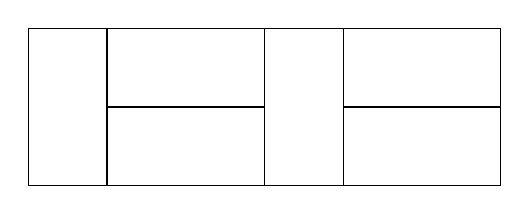
\begin{tikzpicture}
     \draw (0, 0) rectangle (6, 2);
     \draw (1, 0) rectangle (3, 1);
     \draw (1, 1) rectangle (3, 2);
     \draw (4, 0) rectangle (6, 1);
     \draw (4, 1) rectangle (6, 2);
    \end{tikzpicture}
  \end{center}
  The first tile is either vertical (leaving a $2 \times (n-1)$ grid) or horizontal (forcing a second horizontal tile and leaving a $2 \times (n-2)$ grid), so $f_n = f_{n-1} + f_{n-2}$ with $f_0 = f_1 = 1$.

  Define the generating function $F(z) = \sum_{n=0}^\infty f_n z^n$. The recurrence gives
  \[
    F(z) - 1 - z = z(F(z) - 1) + z^2 F(z),
  \]
  so $F(z) = (1 - z - z^2)^{-1}$. Writing $\alpha = \frac{1+\sqrt{5}}{2}$ and $\beta = \frac{1-\sqrt{5}}{2}$ for the roots of $t^2 - t - 1 = 0$, partial fractions give
  \[
    F(z) = \frac{1}{(\alpha - \beta)}\left(\frac{\alpha}{1 - \alpha z} - \frac{\beta}{1 - \beta z}\right),
  \]
  and extracting coefficients yields $f_n = (\alpha^{n+1} - \beta^{n+1})/(\alpha - \beta)$.
\end{eg}

\begin{eg}[Catalan numbers]
  A \emph{Dyck word} of length $2n$ is a string of $n$ opening and $n$ closing brackets that is correctly matched (e.g.\ $(()())$). Let $C_n$ denote the number of Dyck words of length $2n$, with $C_0 = 1$. Every non-empty Dyck word can be uniquely decomposed as $(w_1)w_2$ where $w_1$ and $w_2$ are Dyck words, giving the recurrence
  \[
    C_{n + 1} = \sum_{i = 0}^n C_i\, C_{n - i}.\tag{$*$}
  \]
  Define $c(x) = \sum_{n=0}^\infty C_n x^n$. The convolution in $(*)$ gives $c(x) = 1 + x\,c(x)^2$. Solving and taking the root with $c(0) = 1$,
  \[
    c(x) = \frac{1 - \sqrt{1 - 4x}}{2x},
  \]
  and expanding via the generalised binomial theorem yields $C_n = \frac{1}{n+1}\binom{2n}{n}$.
\end{eg}

\subsubsection*{Sums with a random number of terms}

\begin{thm}[Random sum formula]
  Let $X_1, X_2, \dotsc$ be i.i.d.\ non-negative integer-valued random variables with pgf $p(z)$, and let $N$ be a non-negative integer-valued random variable, independent of the $X_i$, with pgf $h(z)$. Then $S = X_1 + \cdots + X_N$ has pgf
  \[
    p_S(z) = h(p(z)).
  \]
\end{thm}

\begin{proof}
  By the tower property, conditioning on $N$:
  \begin{align*}
    \E[z^{S}] &= \sum_{n = 0}^\infty \P(N = n)\, \E[z^{X_1 + \cdots + X_n}] = \sum_{n = 0}^\infty \P(N = n)\, p(z)^n = h(p(z)).\qedhere
  \end{align*}
\end{proof}

\begin{cor}[Mean and variance of a random sum]
  Under the hypotheses above, if all relevant moments are finite, then
  \[
    \E[S] = \E[N]\,\E[X_1], \qquad \var(S) = \E[N]\,\var(X_1) + (\E[X_1])^2\,\var(N).
  \]
\end{cor}

\begin{proof}
  Differentiating $h(p(z))$ at $z = 1$: $\E[S] = h'(p(1))\,p'(1) = \E[N]\,\E[X_1]$. For the variance, compute $\E[S(S-1)]$ via the second derivative $\frac{\d^2}{\d z^2}h(p(z))\big|_{z=1}$ and use $\var(S) = \E[S(S-1)] + \E[S] - (\E[S])^2$.
\end{proof}


\section{Interesting problems}
\begin{remark}
  In this section we study two important probabilistic processes: branching processes and random walks.
  Both make essential use of probability generating functions.
\end{remark}

\subsection{Branching processes}
\begin{defi}[Branching process]
  A \emph{branching process} is a sequence of random variables $X_0, X_1, X_2, \dotsc$, where $X_n$ denotes the number of individuals in the $n$th generation, satisfying:
  \begin{enumerate}
    \item $X_0 = 1$.
    \item Each individual independently produces $k$ offspring with probability $p_k$, for $k = 0, 1, 2, \dotsc$.
    \item $X_{n+1} = Y_1^{(n)} + Y_2^{(n)} + \cdots + Y_{X_n}^{(n)}$, where $Y_i^{(n)}$ are independent and identically distributed with the same distribution as $X_1$.
  \end{enumerate}
  We write $F(z) = \E[z^{X_1}] = \sum_{k=0}^\infty p_k z^k$ for the \emph{probability generating function} of the offspring distribution, and $F_n(z) = \E[z^{X_n}]$ for the probability generating function of $X_n$.
\end{defi}

\begin{thm}[PGF recursion]
  $F_{n+1}(z) = F(F_n(z)) = F_n(F(z))$.
\end{thm}

\begin{proof}
  \begin{align*}
    F_{n+1}(z)
    &= \E[z^{X_{n+1}}]\\
    &= \E\bigl[\E[z^{X_{n+1}} \mid X_n]\bigr]\\
    &= \sum_{k=0}^\infty \P(X_n = k)\,\E[z^{X_{n+1}} \mid X_n = k]\\
    &= \sum_{k=0}^\infty \P(X_n = k)\,\E[z^{Y_1^{(n)} + \cdots + Y_k^{(n)}}]\\
    &= \sum_{k=0}^\infty \P(X_n = k)\, F(z)^k\\
    &= F_n(F(z)).
  \end{align*}
  Applying this recursion starting from $F_1(z) = F(z)$, we obtain $F_{n+1}(z) = F(F(\cdots F(z) \cdots))$ with $n+1$ applications of $F$, whence $F_{n+1}(z) = F(F_n(z))$ as well.
\end{proof}

\begin{thm}[Mean and variance of a branching process]
  Let $\mu = \E[X_1] = \sum_{k=0}^\infty k\,p_k$ and $\sigma^2 = \var(X_1) < \infty$.
  Then
  \[
    \E[X_n] = \mu^n, \quad \var(X_n) = \sigma^2 \mu^{n-1}(1 + \mu + \mu^2 + \cdots + \mu^{n-1}).
  \]
\end{thm}

\begin{proof}
  By the tower property,
  \[
    \E[X_n] = \E[\E[X_n \mid X_{n-1}]] = \E[\mu X_{n-1}] = \mu\,\E[X_{n-1}].
  \]
  Since $X_0 = 1$, induction gives $\E[X_n] = \mu^n$.

  For the variance, by the tower property,
  \begin{align*}
    \E[X_n^2]
    &= \E[\E[X_n^2 \mid X_{n-1}]]\\
    &= \E[\var(X_n \mid X_{n-1}) + (\E[X_n \mid X_{n-1}])^2]\\
    &= \E[X_{n-1}\,\sigma^2 + \mu^2 X_{n-1}^2]\\
    &= \sigma^2 \mu^{n-1} + \mu^2\,\E[X_{n-1}^2].
  \end{align*}
  Therefore
  \begin{align*}
    \var(X_n)
    &= \E[X_n^2] - \mu^{2n}\\
    &= \mu^2(\E[X_{n-1}^2] - \mu^{2(n-1)}) + \sigma^2 \mu^{n-1}\\
    &= \mu^2\,\var(X_{n-1}) + \sigma^2 \mu^{n-1}.
  \end{align*}
  Iterating and using $\var(X_0) = 0$ gives
  \[
    \var(X_n) = \sigma^2 \mu^{n-1}(1 + \mu + \cdots + \mu^{n-1}). \qedhere
  \]
\end{proof}

\subsubsection*{Extinction probability}
\begin{defi}[Extinction probability]
  The \emph{extinction probability} of a branching process is
  \[
    q = \P\Bigl(\bigcup_{n=1}^\infty \{X_n = 0\}\Bigr) = \lim_{n \to \infty} \P(X_n = 0),
  \]
  where the second equality holds because $\{X_1 = 0\} \subseteq \{X_2 = 0\} \subseteq \cdots$ and by continuity of probability.
\end{defi}

\begin{prop}
  The extinction probability satisfies $F(q) = q$.
\end{prop}

\begin{proof}
  Since $F_n(0) = \sum_{k=0}^\infty \P(X_n = k) \cdot 0^k = \P(X_n = 0)$, we have $q = \lim_{n \to \infty} F_n(0)$.
  By continuity of $F$ on $[0,1]$,
  \[
    F(q) = F\!\left(\lim_{n \to \infty} F_n(0)\right) = \lim_{n \to \infty} F(F_n(0)) = \lim_{n \to \infty} F_{n+1}(0) = q. \qedhere
  \]
\end{proof}

\begin{remark}
  Alternatively, by the law of total probability,
  \[
    q = \sum_{k=0}^\infty p_k\,\P(\text{extinction} \mid X_1 = k) = \sum_{k=0}^\infty p_k\,q^k = F(q),
  \]
  since for the population to go extinct, each of the $k$ independent sub-populations must go extinct, each with probability $q$.
\end{remark}

\begin{thm}[Extinction criterion]
  The extinction probability $q$ is the smallest root of $F(z) = z$ in $[0,1]$.
  If $\mu \leq 1$, then $q = 1$; if $\mu > 1$, then $q < 1$.
\end{thm}

\begin{proof}
  Let $\alpha$ be the smallest root of $F(z) = z$ in $[0,1]$.
  Since $F$ is increasing on $[0,1]$ and $F(0) = p_0 \geq 0$, we have $F(0) \leq \alpha$.
  By monotonicity, $F(F(0)) \leq F(\alpha) = \alpha$.
  Inductively, $F_n(0) \leq \alpha$ for all $n$, so
  \[
    q = \lim_{n \to \infty} F_n(0) \leq \alpha.
  \]
  Since $q$ is itself a root of $F(z) = z$, we conclude $q = \alpha$.

  For the second part, note that $F'(z) \geq 0$ and $F''(z) \geq 0$ for $z \in [0,1]$, so $F$ is increasing and convex.
  Since $F(1) = 1$ and $F'(1) = \mu$:
  \begin{itemize}
    \item If $\mu \leq 1$, then convexity implies $F(z) \geq z$ for all $z \in [0,1]$, so $z = 1$ is the only root.
    \item If $\mu > 1$, then $F$ crosses the line $F = z$ at some $q < 1$.
  \end{itemize}
  \begin{center}
    \begin{tikzpicture}
      \draw (0, 0) -- (4, 0) node [right] {$z$};
      \draw (0, 0) -- (0, 4) node [above] {$F(z)$};
      \draw [dashed] (0, 0) -- (4, 4);
      \draw (0, 2.3) parabola (4, 4);
    \end{tikzpicture}
  \end{center}
\end{proof}

\subsection{Random walk and gambler's ruin}
\begin{defi}[Simple random walk]
  Let $X_1, X_2, \dotsc$ be iid random variables with $\P(X_i = +1) = p$ and $\P(X_i = -1) = q = 1 - p$.
  The sequence $(S_n)_{n \geq 0}$ defined by $S_n = S_0 + X_1 + \cdots + X_n$ is a \emph{simple random walk} starting at $S_0$.
  If $p = q = \frac{1}{2}$, the random walk is \emph{symmetric}.
\end{defi}

\begin{prop}[Gambler's ruin probabilities]
  A gambler starts with $\$z$, where $0 < z < a$, and at each turn wins $\$1$ with probability $p$ or loses $\$1$ with probability $q = 1 - p$.
  Let
  \[
    p_z = \P(\text{walk hits $a$ before $0$} \mid S_0 = z), \quad
    q_z = \P(\text{walk hits $0$ before $a$} \mid S_0 = z).
  \]
  If $p \neq q$, then
  \[
    p_z = \frac{1 - (q/p)^z}{1 - (q/p)^a}, \quad
    q_z = \frac{(q/p)^a - (q/p)^z}{(q/p)^a - 1}.
  \]
  If $p = q = \frac{1}{2}$, then $p_z = z/a$ and $q_z = (a - z)/a$.
  In both cases, $p_z + q_z = 1$, so the game terminates with probability $1$.
\end{prop}

\begin{proof}
  Conditioning on the first step,
  \[
    p_z = p\,p_{z+1} + q\,p_{z-1},
  \]
  for $0 < z < a$, with $p_0 = 0$ and $p_a = 1$.
  Try $p_z = t^z$. Then $pt^2 - t + q = (pt - q)(t - 1) = 0$, with roots $t = 1$ and $t = q/p$.

  If $p \neq q$, the general solution is $p_z = A + B(q/p)^z$.
  From $p_0 = 0$, we get $A = -B$.
  From $p_a = 1$, we obtain $p_z = \frac{1 - (q/p)^z}{1 - (q/p)^a}$.

  If $p = q$, the roots coincide and the general solution is $p_z = A + Bz$, giving $p_z = z/a$.

  The formula for $q_z$ follows by the substitution $p \mapsto q$, $q \mapsto p$, $z \mapsto a - z$ (or directly by $q_z = 1 - p_z$).
\end{proof}

\begin{cor}[Ruin on the infinite line]
  Starting from $z > 0$ with no upper barrier (i.e.\ $a \to \infty$),
  \[
    \P(\text{walk hits $0$ eventually}) = \begin{cases}
      (q/p)^z & \text{if } p > q, \\
      1 & \text{if } p \leq q.
    \end{cases}
  \]
\end{cor}

\begin{proof}
  The events $\{\text{walk hits $0$ before $a$}\}$ increase with $a$, so by continuity of probability,
  \[
    \P(\text{walk hits $0$ eventually}) = \lim_{a \to \infty} q_z,
  \]
  and the result follows from the formulas above.
\end{proof}

\begin{remark}
  If the odds are against the gambler ($p \leq q$), ruin is certain regardless of the initial fortune $z$.
\end{remark}

\subsubsection*{Duration of the game}
\begin{prop}[Expected duration of gambler's ruin]
  Let $D_z$ denote the expected number of steps until the walk is absorbed at $0$ or $a$, starting from $z$.
  Then $D_z < \infty$, and
  \[
    D_z = \begin{cases}
      \dfrac{z}{q - p} - \dfrac{a}{q - p} \cdot \dfrac{1 - (q/p)^z}{1 - (q/p)^a} & \text{if } p \neq q, \\[8pt]
      z(a - z) & \text{if } p = q = \frac{1}{2}.
    \end{cases}
  \]
\end{prop}

\begin{proof}
  We first show $D_z < \infty$.
  In any block of $a$ consecutive steps, the probability of all steps being $+1$ or all being $-1$ is at least $p^a + q^a > 0$, which guarantees absorption.
  Hence $D_z \leq \frac{a}{p^a + q^a} < \infty$.

  Conditioning on the first step,
  \[
    D_z = 1 + p\,D_{z+1} + q\,D_{z-1},
  \]
  with $D_0 = D_a = 0$.

  \emph{Case $p \neq q$.}
  For a particular solution, try $D_z = Cz$: substituting gives $C = \frac{1}{q - p}$.
  The complementary equation $pt^2 - t + q = 0$ has roots $1$ and $q/p$, so the general solution is
  \[
    D_z = A + B\left(\frac{q}{p}\right)^z + \frac{z}{q - p}.
  \]
  Applying $D_0 = D_a = 0$ yields the stated formula.

  \emph{Case $p = q = \frac{1}{2}$.}
  Try $D_z = Cz^2$: substituting gives $C = -1$.
  The general solution is $D_z = -z^2 + A + Bz$, and the boundary conditions give $D_z = z(a - z)$.
\end{proof}

\begin{eg}[Generating function approach to gambler's ruin]
  Let $U_{z,n} = \P(\text{walk absorbed at $0$ at step $n$} \mid S_0 = z)$, and define the generating function
  \[
    U_z(s) = \sum_{n=0}^\infty U_{z,n}\,s^n.
  \]
  The boundary conditions are $U_{0,0} = 1$, $U_{z,0} = 0$ for $0 < z \leq a$, and $U_{0,n} = U_{a,n} = 0$ for $n > 0$.

  From the recurrence $U_{z,n+1} = p\,U_{z+1,n} + q\,U_{z-1,n}$, multiplying by $s^{n+1}$ and summing over $n \geq 0$ gives
  \[
    U_z(s) = ps\,U_{z+1}(s) + qs\,U_{z-1}(s).
  \]
  Trying $U_z(s) = \lambda(s)^z$ leads to $ps\,\lambda^2 - \lambda + qs = 0$, with roots
  \[
    \lambda_1(s),\, \lambda_2(s) = \frac{1 \pm \sqrt{1 - 4pqs^2}}{2ps}.
  \]
  The general solution $U_z(s) = A(s)\,\lambda_1(s)^z + B(s)\,\lambda_2(s)^z$, together with $U_0(s) = 1$ and $U_a(s) = 0$, gives
  \[
    U_z(s) = \frac{\lambda_1(s)^a\,\lambda_2(s)^z - \lambda_2(s)^a\,\lambda_1(s)^z}{\lambda_1(s)^a - \lambda_2(s)^a}.
  \]
  Since $\lambda_1(s)\,\lambda_2(s) = q/p$, this simplifies to
  \[
    U_z(s) = \left(\frac{q}{p}\right)^z \cdot \frac{\lambda_1(s)^{a-z} - \lambda_2(s)^{a-z}}{\lambda_1(s)^a - \lambda_2(s)^a}.
  \]
  One can verify $U_z(1) = q_z$.
  Similarly, if $V_z(s)$ is the generating function for absorption at $a$, then the expected duration is $D_z = U_z'(1) + V_z'(1)$.
\end{eg}
\section{Continuous random variables}
\subsection{Continuous random variables}
\begin{eg}
  Consider throwing a needle randomly onto the ground and recording the angle it makes with a fixed horizontal.
  The sample space is $\Omega = \{\omega \in \R : 0 \leq \omega < 2\pi\}$, and
  \[
    \P(\omega \in [0, \theta]) = \frac{\theta}{2\pi}, \quad 0 \leq \theta \leq 2\pi.
  \]
  We cannot assign nonzero probability to any single outcome.
\end{eg}

\begin{remark}
  For continuous distributions, we describe probabilities via a \emph{probability density function} $f$: for small $\delta x$,
  \[
    \P(X \in [x, x + \delta x]) = f(x)\,\delta x + o(\delta x).
  \]
  Integrating, $\P(X \in [a, b]) = \int_a^b f(x)\;\d x$.
\end{remark}

\begin{defi}[Continuous random variable]
  A random variable $X : \Omega \to \R$ is \emph{continuous} if there is a function $f : \R \to \R_{\geq 0}$ such that
  \[
    \P(a \leq X \leq b) = \int_a^b f(x) \;\d x.
  \]
  We call $f$ the \emph{probability density function} (pdf), which satisfies
  \begin{itemize}
    \item $f \geq 0$;
    \item $\int_{-\infty}^\infty f(x)\;\d x = 1$.
  \end{itemize}
\end{defi}

\begin{remark}
  For any continuous random variable, $\P(X = a) = 0$ since $\int_a^a f(x)\;\d x = 0$.
  Hence $\P\bigl(\bigcup_{a \in \Q} [X = a]\bigr) = 0$ by countable additivity.
\end{remark}

\begin{defi}[Cumulative distribution function]
  The \emph{cumulative distribution function} (cdf) of a random variable $X$ (discrete, continuous, or neither) is
  \[
    F(x) = \P(X \leq x).
  \]
\end{defi}

\begin{remark}
  The cdf $F$ is non-decreasing, with $F(x) \to 0$ as $x \to -\infty$ and $F(x) \to 1$ as $x \to \infty$.
  For a continuous random variable,
  \[
    F(x) = \int_{-\infty}^x f(z)\;\d z,
  \]
  so $F$ is continuous and differentiable, with $F'(x) = f(x)$.
  The name ``continuous random variable'' reflects the (absolute) continuity of $F$.
\end{remark}

\begin{eg}
  The cdf of a continuous random variable might look like this:
  \begin{center}
    \begin{tikzpicture}
      \draw [->] (0, 0) -- (3, 0);
      \draw [->] (0, 0) -- (0, 2) node [above] {$\P$};
      \draw (0, 0) parabola (2.5, 1.5);
    \end{tikzpicture}
  \end{center}
  The cdf of a discrete random variable might look like this:
  \begin{center}
    \begin{tikzpicture}
      \draw [->] (0, 0) -- (3, 0);
      \draw [->] (0, 0) -- (0, 2) node [above] {$\P$};
      \draw (0, 0) -- (1, 0) -- (1, 0.5) -- (2, 0.5) -- (2, 1) -- (3, 1) -- (3, 1.5);
    \end{tikzpicture}
  \end{center}
  The cdf of a random variable that is neither discrete nor continuous might look like this:
  \begin{center}
    \begin{tikzpicture}
      \draw [->] (0, 0) -- (3, 0);
      \draw [->] (0, 0) -- (0, 2) node [above] {$\P$};
      \draw (0, 0) parabola (1, 1);
      \draw (1, 1) -- (2.5, 1) -- (2.5, 2);
      \node [circ] at (2.5, 2) {};
    \end{tikzpicture}
  \end{center}
\end{eg}

\begin{remark}
  For any random variable, $\P(a < X \leq b) = F(b) - F(a)$.
  For continuous random variables, this equals $\int_a^b f(x)\;\d x$.
\end{remark}

\begin{defi}[Uniform distribution]
  The \emph{uniform distribution} on $[a, b]$ has pdf
  \[
    f(x) = \frac{1}{b - a}, \quad a \leq x \leq b,
  \]
  and cdf $F(x) = \frac{x - a}{b - a}$ for $a \leq x \leq b$.
  We write $X \sim U[a, b]$.
\end{defi}

\begin{defi}[Exponential distribution]
  The \emph{exponential distribution with parameter $\lambda > 0$} has pdf $f(x) = \lambda e^{-\lambda x}$ and cdf $F(x) = 1 - e^{-\lambda x}$ for $x \geq 0$.
  We write $X \sim \mathcal{E}(\lambda)$.
\end{defi}

\begin{prop}[Memoryless property]
  The exponential distribution is \emph{memoryless}:
  \[
    \P(X \geq x + z \mid X \geq x) = \P(X \geq z).
  \]
\end{prop}

\begin{proof}
  \begin{align*}
    \P(X \geq x + z \mid X \geq x) &= \frac{\P(X \geq x + z)}{\P(X \geq x)}\\
    &= \frac{e^{-\lambda(x + z)}}{e^{-\lambda x}}\\
    &= e^{-\lambda z}\\
    &= \P(X \geq z).\qedhere
  \end{align*}
\end{proof}

\begin{remark}
  The geometric distribution is the discrete analogue: it is the unique discrete memoryless distribution.
\end{remark}

\begin{defi}[Hazard rate]
  The \emph{hazard rate} of a continuous random variable with pdf $f$ and cdf $F$ is
  \[
    h(x) = \frac{f(x)}{1 - F(x)}.
  \]
  This satisfies $\P(x \leq X \leq x + \delta x \mid X \geq x) = h(x)\,\delta x + o(\delta x)$.
\end{defi}

\begin{remark}
  The exponential distribution has constant hazard rate $h(x) = \lambda$.
\end{remark}

\begin{defi}[Expectation]
  The \emph{expectation} (or \emph{mean}) of a continuous random variable $X$ is
  \[
    \E[X] = \int_{-\infty}^\infty x\,f(x)\;\d x,
  \]
  provided $\int_0^\infty x\,f(x)\;\d x$ and $\int_{-\infty}^0 x\,f(x)\;\d x$ are not both infinite.
\end{defi}

\begin{thm}[Tail sum formula]
  If $X$ is a continuous random variable, then
  \[
    \E[X] = \int_0^\infty \P(X \geq x)\;\d x - \int_0^\infty \P(X \leq -x)\;\d x.
  \]
\end{thm}

\begin{remark}
  In the discrete case, this becomes $\sum_{x=0}^\infty x\,\P(X = x) = \sum_{x=0}^\infty \P(X > x)$, since both sides contain $x$ copies of $\P(X = x)$.
\end{remark}

\begin{proof}
  \begin{align*}
    \int_0^\infty \P(X \geq x)\;\d x &= \int_0^\infty \int_x^\infty f(y)\;\d y\;\d x\\
    &= \int_0^\infty \int_0^\infty I[y \geq x]\,f(y)\;\d y\;\d x\\
    &= \int_0^\infty \left(\int_0^\infty I[x \leq y]\;\d x\right) f(y)\;\d y\\
    &= \int_0^\infty y\,f(y)\;\d y.
  \end{align*}
  Similarly, $\int_0^\infty \P(X \leq -x)\;\d x = -\int_{-\infty}^0 y\,f(y)\;\d y$.
\end{proof}

\begin{eg}
  If $X \sim \mathcal{E}(\lambda)$, then $\P(X \geq x) = e^{-\lambda x}$, so
  \[
    \E[X] = \int_0^\infty e^{-\lambda x}\;\d x = \frac{1}{\lambda}.
  \]
\end{eg}

\begin{defi}[Variance]
  The \emph{variance} of a continuous random variable $X$ is
  \[
    \var(X) = \E[(X - \E[X])^2] = \E[X^2] - (\E[X])^2.
  \]
\end{defi}

\begin{eg}
  Let $X \sim U[a, b]$. Then
  \[
    \E[X] = \int_a^b \frac{x}{b - a}\;\d x = \frac{a + b}{2},
  \]
  and
  \[
    \var(X) = \int_a^b \frac{x^2}{b - a}\;\d x - (\E[X])^2 = \frac{(b - a)^2}{12}.
  \]
\end{eg}

\begin{defi}[Mode and median]
  Given a pdf $f$, a value $\hat{x}$ is a \emph{mode} if $f(\hat{x}) \geq f(x)$ for all $x$.

  A value $\hat{x}$ is a \emph{median} if
  \[
    \int_{-\infty}^{\hat{x}} f(x)\;\d x = \frac{1}{2} = \int_{\hat{x}}^\infty f(x)\;\d x.
  \]
  For a discrete random variable, $\hat{x}$ is a median if $\P(X \leq \hat{x}) \geq \frac{1}{2}$ and $\P(X \geq \hat{x}) \geq \frac{1}{2}$.
\end{defi}

\begin{defi}[Sample mean]
  If $X_1, \dotsc, X_n$ is a random sample from some distribution, the \emph{sample mean} is
  \[
    \bar{X} = \frac{1}{n} \sum_{i=1}^n X_i.
  \]
\end{defi}

\subsection{Stochastic ordering and inspection paradox}
\begin{defi}[Stochastic order]
  We write $X \geq_{\mathrm{st}} Y$ (\emph{stochastic order}) if $\P(X > t) \geq \P(Y > t)$ for all $t$.
\end{defi}

\begin{remark}
  Stochastic order is transitive.
  It implies expectation ordering: if $X \geq_{\mathrm{st}} Y$, then
  \[
    \E[X] = \int_0^\infty \P(X > x)\;\d x \geq \int_0^\infty \P(Y > x)\;\d x = \E[Y].
  \]
  The converse is false: $\E[X] \geq \E[Y]$ does not imply $X \geq_{\mathrm{st}} Y$.
\end{remark}

\begin{eg}[Inspection paradox]
  Suppose $n$ families have children attending a school.
  Family $i$ has $X_i$ children at the school, where $X_1, \dotsc, X_n$ are iid with $\P(X_i = k) = p_k$ and mean $\mu$.

  Pick a child at random, and let $J$ be the index of the family from which they come. Then
  \[
    \P(X_J = k \mid J = j) = \frac{\P(J = j,\, X_j = k)}{\P(J = j)}.
  \]
  The denominator is $1/n$.
  The numerator requires the $j$th family to have $k$ members (probability $p_k$) and that we picked a member from that family (probability $\E\bigl[\frac{k}{k + \sum_{i \neq j} X_i}\bigr]$).
  So
  \[
    \P(X_J = k \mid J = j) = \E\left[\frac{nkp_k}{k + \sum_{i \neq j} X_i}\right],
  \]
  which is independent of $j$.
  Hence
  \[
    \frac{\P(X_J = k)}{\P(X_1 = k)} = \E\left[\frac{nk}{k + \sum_{i \neq j} X_i}\right].
  \]
  This ratio is increasing in $k$ and exceeds $1$ for $k > \mu$, so $X_J \geq_{\mathrm{st}} X_1$: the family size of a randomly chosen child is stochastically larger than the family size of a randomly chosen family.
\end{eg}

\subsection{Jointly distributed random variables}
\begin{defi}[Joint distribution]
  Two random variables $X, Y$ have \emph{joint distribution} $F \colon \R^2 \to [0, 1]$ defined by
  \[
    F(x, y) = \P(X \leq x,\, Y \leq y).
  \]
  The \emph{marginal distribution} of $X$ is
  \[
    F_X(x) = \P(X \leq x) = \P(X \leq x,\, Y < \infty) = F(x, \infty) = \lim_{y \to \infty} F(x, y).
  \]
\end{defi}

\begin{defi}[Joint pdf]
  We say $X_1, \dotsc, X_n$ are \emph{jointly continuous random variables} with \emph{joint pdf} $f$ if for any $A \subseteq \R^n$,
  \[
    \P((X_1, \dotsc, X_n) \in A) = \int_{(x_1, \dotsc, x_n) \in A} f(x_1, \dotsc, x_n)\;\d x_1 \dotsm \d x_n,
  \]
  where $f(x_1, \dotsc, x_n) \geq 0$ and
  \[
    \int_{\R^n} f(x_1, \dotsc, x_n)\;\d x_1 \dotsm \d x_n = 1.
  \]
\end{defi}

\begin{eg}
  When $n = 2$,
  \[
    F(x, y) = \P(X \leq x,\, Y \leq y) = \int_{-\infty}^x \int_{-\infty}^y f(s, t)\;\d t\;\d s.
  \]
  If $F$ is differentiable, then
  \[
    f(x, y) = \frac{\partial^2}{\partial x\,\partial y} F(x, y).
  \]
\end{eg}

\begin{thm}
  If $X$ and $Y$ are jointly continuous random variables, then they are individually continuous random variables.
\end{thm}

\begin{proof}
  We show that $X$ has a density function.
  \begin{align*}
    \P(X \in A) &= \P(X \in A,\, Y \in (-\infty, +\infty))\\
    &= \int_{x \in A} \int_{-\infty}^\infty f(x, y)\;\d y\;\d x\\
    &= \int_{x \in A} f_X(x)\;\d x,
  \end{align*}
  where
  \[
    f_X(x) = \int_{-\infty}^\infty f(x, y)\;\d y
  \]
  is the marginal pdf of $X$.
\end{proof}

\begin{defi}[Independent continuous random variables]
  Continuous random variables $X_1, \dotsc, X_n$ are \emph{independent} if
  \[
    \P(X_1 \in A_1,\, X_2 \in A_2,\, \dotsc,\, X_n \in A_n) = \P(X_1 \in A_1)\P(X_2 \in A_2) \dotsm \P(X_n \in A_n)
  \]
  for all $A_i \subseteq \Omega_{X_i}$.
  Equivalently, letting $F_{X_i}$ and $f_{X_i}$ denote the cdf and pdf of $X_i$,
  \[
    F(x_1, \dotsc, x_n) = F_{X_1}(x_1) \dotsm F_{X_n}(x_n)
    \quad\text{or}\quad
    f(x_1, \dotsc, x_n) = f_{X_1}(x_1) \dotsm f_{X_n}(x_n).
  \]
\end{defi}

\begin{remark}
  To verify independence, it suffices to factorise the joint pdf into factors each involving only one variable.
\end{remark}

\begin{eg}
  If $(X_1, X_2)$ is uniform on $[0, 1]^2$, then $f(x_1, x_2) = 1 = f_{X_1}(x_1) \cdot f_{X_2}(x_2)$, so $X_1$ and $X_2$ are independent.

  If instead $(Y_1, Y_2)$ is uniform on $\{(y_1, y_2) \in [0, 1]^2 : y_1 \leq y_2\}$, then $f(y_1, y_2) = 2\, \mathbf{1}[y_1 \leq y_2]$, which does not factorise, so $Y_1$ and $Y_2$ are not independent.
\end{eg}

\begin{prop}
  For independent continuous random variables $X_1, \dotsc, X_n$,
  \begin{enumerate}
    \item $\E[\prod_i X_i] = \prod_i \E[X_i]$;
    \item $\var(\sum_i X_i) = \sum_i \var(X_i)$.
  \end{enumerate}
\end{prop}

\subsection{Geometric probability}
\begin{eg}
  Two points $X$ and $Y$ are chosen independently and uniformly on a line segment of length $L$.
  What is the probability that $|X - Y| \leq \ell$?
  Since each of $X$ and $Y$ has pdf $1/L$, the joint pdf is
  \[
    f(x, y) = \frac{1}{L^2}.
  \]
  \begin{center}
    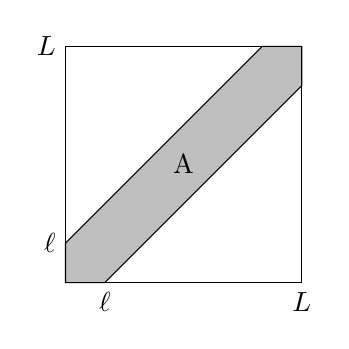
\begin{tikzpicture}
      \draw (0, 0) rectangle (3, 3);
      \draw [fill=gray!50!white] (0, 0) -- (0.5, 0) -- (3, 2.5) -- (3, 3) -- (2.5, 3) -- (0, 0.5) -- cycle;
      \node at (1.5, 1.5) {A};
      \node at (0.5, 0) [below] {$\ell$};
      \node at (3, 0) [below] {$L$};
      \node at (0, 0.5) [left] {$\ell$};
      \node at (0, 3) [left] {$L$};
    \end{tikzpicture}
  \end{center}
  The shaded region $A$ is where $|x - y| \leq \ell$.
  The unshaded region is a square of side $L - \ell$, so the area of $A$ is $L^2 - (L - \ell)^2 = 2L\ell - \ell^2$.
  Hence
  \[
    \P(|X - Y| \leq \ell) = \int_A f(x, y)\;\d x\;\d y = \frac{2L\ell - \ell^2}{L^2}.
  \]
\end{eg}

\begin{eg}[Bertrand's paradox]
  What is the probability that a random chord of a circle is longer than the side of an inscribed equilateral triangle?

  There are three natural interpretations of ``random chord''.
  \begin{enumerate}
    \item Pick two endpoints independently and uniformly on the circumference.
      Draw the inscribed triangle with one vertex at an endpoint.
      The chord is longer than a side of the triangle if and only if the other endpoint lies between the two remaining vertices, which happens with probability $1/3$.
      \begin{center}
        \begin{tikzpicture}
          \draw circle [radius = 1];
          \draw (0, 1) -- (0.866, -0.5) -- (-0.866, -0.5) -- cycle;
          \node [circ, fill=red] at (0, 1) {};
          \draw [mblue] (0, 1) -- (-1, 0);
          \draw [mred] (0, 1) -- (0, -1);
          \draw [mblue] (0, 1) -- (1, 0);
        \end{tikzpicture}
      \end{center}
    \item WLOG the chord is horizontal, on the lower side of the circle.
      The midpoint is uniformly distributed along the dashed line.
      The chord is long if and only if the midpoint lies in the lower half, giving probability $1/2$.
      \begin{center}
        \begin{tikzpicture}
          \draw circle [radius = 1];
          \draw (0, 1) -- (0.866, -0.5) -- (-0.866, -0.5) -- cycle;
          \node [circ, fill=mred] at (0, 1) {};
          \draw [dashed] (0, 1) -- (0, -1);
          \draw [mblue] (-0.4359, -0.9) -- (0.4359, -0.9);
          \draw [mblue] (-0.8, -0.6) -- (0.8, -0.6);
          \draw [mred] (-0.9539, -0.3) -- (0.9539, -0.3);
          \draw [mred] (-1, 0) -- (1, 0);
        \end{tikzpicture}
      \end{center}
    \item The midpoint of the chord is uniformly distributed over the disc.
      The chord is long if and only if the midpoint lies in the inscribed circle of half the radius, giving probability $1/4$.
       \begin{center}
        \begin{tikzpicture}
          \draw circle [radius = 1];
          \draw (0, 1) -- (0.866, -0.5) -- (-0.866, -0.5) -- cycle;
          \node [circ, fill=mred] at (0, 1) {};
          \draw circle [radius = 0.5];
          \draw [mred] (0, -1) -- (-0.6, 0.8);
          \draw [mblue] (-0.9539, 0.3) -- (0.4359, 0.9);
          \draw [mblue] (0.6, -0.8) -- (0.9165, 0.4);
          \draw [mblue] (-1, 0) -- (0.3, -0.9539);
        \end{tikzpicture}
      \end{center}
  \end{enumerate}
  The three interpretations give different answers.
  This illustrates why one must specify the probability model precisely when saying ``at random''.
\end{eg}

\begin{eg}[Buffon's needle]
  A needle of length $\ell$ is tossed at random onto a floor marked with parallel lines a distance $L$ apart, where $\ell \leq L$.
  Let $A$ be the event that the needle intersects a line.
  \begin{center}
    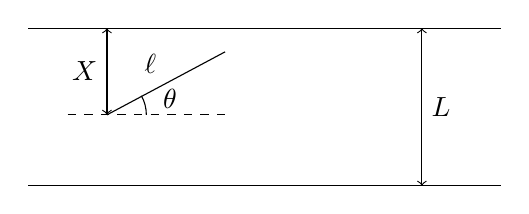
\begin{tikzpicture}
      \draw (-3, -1) -- (3, -1);
      \draw (-3, 1) -- (3, 1);
      \draw (-2, -0.1) -- (-0.5, 0.7) node [anchor = south east, pos = 0.5] {$\ell$};
      \draw [->] (-2, -0.1) -- (-2, 1) node [left, pos = 0.5] {$X$};
      \draw [->] (-2, 1) -- (-2, -0.1);
      \draw [dashed] (-2.5, -0.1) -- (-0.5, -0.1);
      \draw (-1.5, -0.1) arc (0:29:0.5);
      \node at (-1.2, 0.1) {$\theta$};
      \draw [->] (2, -1) -- (2, 1) node [right, pos = 0.5] {$L$};
      \draw [->] (2, 1) -- (2, -1);
    \end{tikzpicture}
  \end{center}
  Let $X \sim U[0, L]$ be the distance from the needle's centre to the nearest line, and $\theta \sim U[0, \pi]$ the angle of the needle.
  Since $X$ and $\theta$ are independent,
  \[
    f(x, \theta) = \frac{1}{L\pi}.
  \]
  The needle touches a line if and only if $X \leq \ell \sin \theta$, so
  \[
    \P(A) = \int_{\theta = 0}^\pi \underbrace{\frac{\ell \sin \theta}{L}}_{\P(X \leq \ell \sin \theta)} \frac{1}{\pi}\;\d \theta = \frac{2\ell}{\pi L}.
  \]
  Since the answer involves $\pi$, one can estimate $\pi$ by repeated experiment.
  If $N$ out of $n$ tosses produce a hit, then $\hat{p} = N/n$ estimates $p = \P(A)$, giving
  \[
    \hat{\pi} = \frac{2\ell}{\hat{p}L}.
  \]
  We will later see that this is an inefficient estimator of $\pi$.
\end{eg}
\subsection{The normal distribution}
\begin{defi}[Normal distribution]
  The \emph{normal distribution} with parameters $\mu, \sigma^2$, written $N(\mu, \sigma^2)$, has pdf
  \[
    f(x) = \frac{1}{\sqrt{2\pi}\,\sigma}\exp\left(-\frac{(x - \mu)^2}{2\sigma^2}\right),
  \]
  for $x \in \R$.
  \begin{center}
    \begin{tikzpicture}[yscale=1.5]
      \draw (-3, 0) -- (3, 0);
      \draw (0, 1.3) -- (0, 0) node [below] {$\mu$};
      \draw [domain=-3:3,samples=50, mblue] plot (\x, {exp(-\x * \x)});
    \end{tikzpicture}
  \end{center}
  The \emph{standard normal} is $N(0, 1)$.
  We write $\phi(x)$ for its pdf and $\Phi(x)$ for its cdf.
\end{defi}

\begin{remark}
  The normal distribution is of central importance, largely because of the central limit theorem: the average of a large number of iid random variables is approximately normal.
  By symmetry, the mode and median of $N(\mu, \sigma^2)$ are both $\mu$.
\end{remark}

\begin{prop}[Normalisation]
  \[
    \int_{-\infty}^\infty \frac{1}{\sqrt{2\pi\sigma^2}}\, e^{-(x - \mu)^2 / 2\sigma^2}\;\d x = 1.
  \]
\end{prop}

\begin{proof}
  Substituting $z = (x - \mu)/\sigma$ gives
  \[
    I = \int_{-\infty}^\infty \frac{1}{\sqrt{2\pi}}\,e^{-z^2/2}\;\d z.
  \]
  Then
  \begin{align*}
    I^2 &= \int_{-\infty}^\infty \frac{1}{\sqrt{2\pi}}\, e^{-x^2/2}\;\d x \int_{-\infty}^\infty \frac{1}{\sqrt{2\pi}}\, e^{-y^2/2}\;\d y\\
    &= \int_0^\infty \int_0^{2\pi} \frac{1}{2\pi}\,e^{-r^2/2}\,r\;\d\theta\;\d r\\
    &= 1.\qedhere
  \end{align*}
\end{proof}

\begin{prop}
  If $X \sim N(\mu, \sigma^2)$, then $\E[X] = \mu$.
\end{prop}

\begin{proof}
  \begin{align*}
    \E[X] &= \frac{1}{\sqrt{2\pi}\,\sigma} \int_{-\infty}^\infty x\, e^{-(x - \mu)^2/2\sigma^2}\;\d x\\
    &= \frac{1}{\sqrt{2\pi}\,\sigma}\int_{-\infty}^\infty (x - \mu)\,e^{-(x - \mu)^2/2\sigma^2}\;\d x + \frac{\mu}{\sqrt{2\pi}\,\sigma}\int_{-\infty}^\infty e^{-(x - \mu)^2/2\sigma^2}\;\d x.
  \end{align*}
  The first integral vanishes by antisymmetry about $\mu$; the second equals $\mu$ by normalisation.
\end{proof}

\begin{prop}
  If $X \sim N(\mu, \sigma^2)$, then $\var(X) = \sigma^2$.
\end{prop}

\begin{proof}
  Substituting $Z = (X - \mu)/\sigma$ gives $\E[Z] = 0$ and $\var(X) = \sigma^2 \var(Z)$.
  By integration by parts,
  \begin{align*}
    \var(Z) &= \frac{1}{\sqrt{2\pi}} \int_{-\infty}^\infty z^2 e^{-z^2/2}\;\d z\\
    &= \left[-\frac{1}{\sqrt{2\pi}}\,z\,e^{-z^2/2}\right]_{-\infty}^\infty + \frac{1}{\sqrt{2\pi}}\int_{-\infty}^\infty e^{-z^2/2}\;\d z\\
    &= 0 + 1 = 1.
  \end{align*}
  Hence $\var(X) = \sigma^2$.
\end{proof}

\begin{eg}
  UK adult male heights are normally distributed with mean $70''$ and standard deviation $3''$.
  In the Netherlands, these figures are $71''$ and $3''$.

  Let $X \sim N(70, 9)$ and $Y \sim N(71, 9)$ be the heights of randomly chosen UK and Dutch males, respectively.
  Then (as we will show later) $Y - X \sim N(1, 18)$, so
  \[
    \P(Y > X) = \P\left(\frac{Y - X - 1}{\sqrt{18}} > \frac{-1}{\sqrt{18}}\right) = 1 - \Phi(-1/\sqrt{18}) \approx 0.5931.
  \]

  Now suppose that in both countries, Olympic basketball players are selected from males whose height exceeds the mean by at least $4''$ (the tallest $9.1\%$).
  Then
  \[
    \P(Y > X \mid X \geq 74,\, Y \geq 75) = \frac{\int_{x = 74}^{75} \phi_X(x)\;\d x + \int_{x = 75}^\infty \int_{y=x}^\infty \phi_Y(y)\,\phi_X(x)\;\d y\;\d x}{\int_{x=74}^\infty \phi_X(x)\;\d x \int_{y=75}^\infty \phi_Y(y)\;\d y} \approx 0.7558.
  \]
  Although the means differ by only $1''$, conditioning on the upper tails greatly amplifies the difference.
\end{eg}

\subsection{Transformation of random variables}
\subsubsection*{Single random variable}
\begin{thm}
  Let $X$ be a continuous random variable with pdf $f_X$.
  If $h$ is continuous and strictly increasing with $h^{-1}$ differentiable, then $Y = h(X)$ has pdf
  \[
    f_Y(y) = f_X(h^{-1}(y))\,\frac{\d}{\d y}h^{-1}(y).
  \]
\end{thm}

\begin{proof}
  \begin{align*}
    F_Y(y) &= \P(Y \leq y) = \P(h(X) \leq y) = \P(X \leq h^{-1}(y)) = F_X(h^{-1}(y)).
  \end{align*}
  Differentiating with respect to $y$ gives the result.
\end{proof}

\begin{remark}
  It is often easier to redo this proof than to remember the formula.
\end{remark}

\begin{eg}
  Let $X \sim U[0, 1]$ and $Y = -\log X$. Then
  \begin{align*}
    \P(Y \leq y) &= \P(-\log X \leq y) = \P(X \geq e^{-y}) = 1 - e^{-y},
  \end{align*}
  which is the cdf of $\mathcal{E}(1)$.
\end{eg}

\begin{thm}[Inverse transform sampling]
  Let $U \sim U[0, 1]$.
  For any strictly increasing cdf $F$, the random variable $X = F^{-1}(U)$ has distribution function $F$.
\end{thm}

\begin{proof}
  \[
    \P(X \leq x) = \P(F^{-1}(U) \leq x) = \P(U \leq F(x)) = F(x).\qedhere
  \]
\end{proof}

\begin{remark}
  If $F$ is not strictly increasing, we define $F^{-1}(u) = \inf\{x : F(x) \geq u\}$ for $0 < u < 1$, and the same result holds.
  For discrete random variables with $\P(X = x_i) = p_i$, the analogous construction sets $X = x_j$ when $\sum_{i=0}^{j-1} p_i \leq U < \sum_{i=0}^{j} p_i$.
\end{remark}

\subsubsection*{Multiple random variables}
Suppose $X_1, \dotsc, X_n$ have joint pdf $f$, and let
\begin{align*}
  Y_1 &= r_1(X_1, \dotsc, X_n),\\
  Y_2 &= r_2(X_1, \dotsc, X_n),\\
  &\;\;\vdots \\
  Y_n &= r_n(X_1, \dotsc, X_n).
\end{align*}
Let $R \subseteq \R^n$ with $\P((X_1, \dotsc, X_n) \in R) = 1$, and suppose the map $r \colon R \to S$ is bijective with inverse
\begin{align*}
  X_1 &= s_1(Y_1, \dotsc, Y_n),\\
  X_2 &= s_2(Y_1, \dotsc, Y_n),\\
  &\;\;\vdots\\
  X_n &= s_n(Y_1, \dotsc, Y_n).
\end{align*}

\begin{defi}[Jacobian determinant]
  Suppose $\frac{\partial s_i}{\partial y_j}$ exists and is continuous for all $(y_1, \dotsc, y_n) \in S$. The \emph{Jacobian determinant} is
  \[
    J = \frac{\partial(s_1, \dotsc, s_n)}{\partial(y_1, \dotsc, y_n)} =
    \det
    \begin{pmatrix}
      \frac{\partial s_1}{\partial y_1} & \cdots & \frac{\partial s_1}{\partial y_n}\\
      \vdots & \ddots & \vdots\\
      \frac{\partial s_n}{\partial y_1} & \cdots & \frac{\partial s_n}{\partial y_n}
    \end{pmatrix}
  \]
\end{defi}

\begin{prop}
  $(Y_1, \dotsc, Y_n)$ has pdf
  \[
    g(y_1, \dotsc, y_n) = f(s_1(y_1, \dotsc, y_n), \dotsc, s_n(y_1, \dotsc, y_n))\,|J|
  \]
  for $(y_1, \dotsc, y_n) \in S$, and $0$ otherwise.
\end{prop}

\begin{proof}
  For $A \subseteq R$ with image $B = r(A)$, the change of variables formula gives
  \begin{align*}
    \P((X_1, \dotsc, X_n) \in A) &= \int_A f(x_1, \dotsc, x_n)\;\d x_1 \dotsm \d x_n\\
    &= \int_B f(s_1(y_1, \dotsc, y_n), \dotsc, s_n(y_1, \dotsc, y_n))\,|J|\;\d y_1 \dotsm \d y_n\\
    &= \P((Y_1, \dotsc, Y_n) \in B).\qedhere
  \end{align*}
\end{proof}

\begin{eg}
  Suppose $(X, Y)$ has pdf
  \[
    f(x, y) =
    \begin{cases}
      4xy & 0 \leq x \leq 1,\; 0 \leq y \leq 1\\
      0 & \text{otherwise.}
    \end{cases}
  \]
  Note that $X$ and $Y$ are independent, each with pdf $f(x) = 2x$.

  Define $U = X/Y$, $V = XY$, so $X = \sqrt{UV}$ and $Y = \sqrt{V/U}$.
  The Jacobian is
  \[
    J = \det
    \begin{pmatrix}
      \partial x/\partial u & \partial x/\partial v\\
      \partial y/\partial u & \partial y/\partial v
    \end{pmatrix}
    =
    \det
    \begin{pmatrix}
      \frac{1}{2}\sqrt{v/u} & \frac{1}{2}\sqrt{u/v}\\
      -\frac{1}{2}\sqrt{v/u^3} & \frac{1}{2}\sqrt{1/(uv)}
    \end{pmatrix}
    = \frac{1}{2u}.
  \]
  Alternatively, the forward Jacobian is
  \[
    \det
    \begin{pmatrix}
      \partial u/\partial x & \partial u/\partial y\\
      \partial v/\partial x & \partial v/\partial y
    \end{pmatrix} = 2u,
  \]
  so $|J| = 1/(2u)$.
  Hence
  \[
    g(u, v) = 4\sqrt{uv}\sqrt{\frac{v}{u}} \cdot \frac{1}{2u} = \frac{2v}{u}\,\mathbf{1}[(u, v) \in S].
  \]
  Since this does not factorise, $U$ and $V$ are not independent.
\end{eg}

\begin{remark}
  In the linear case $\mathbf{Y} = A\mathbf{X}$ with $A$ invertible, we have $\mathbf{X} = A^{-1}\mathbf{Y}$ and $|J| = |\det A|^{-1}$, so
  \[
    g(y_1, \dotsc, y_n) = \frac{1}{|\det A|}\,f(A^{-1}\mathbf{y}).
  \]
\end{remark}

\begin{eg}
  Let $X_1, X_2$ have joint pdf $f$.
  To find the pdf of $Y = X_1 + X_2$, introduce $Z = X_2$, so
  \[
    \begin{pmatrix}
      Y\\
      Z
    \end{pmatrix} =
    \begin{pmatrix}
      1 & 1 \\
      0 & 1
    \end{pmatrix}
    \begin{pmatrix}
      X_1\\
      X_2
    \end{pmatrix}.
  \]
  Since $|\det A| = 1$, the joint pdf of $(Y, Z)$ is $g(y, z) = f(y - z, z)$, and marginalising gives
  \[
    f_Y(y) = \int_{-\infty}^\infty f(y - z, z)\;\d z.
  \]
  If $X_1$ and $X_2$ are independent with pdfs $f_1, f_2$, this becomes the \emph{convolution}
  \[
    f_Y(y) = \int_{-\infty}^\infty f_1(y - z)\, f_2(z)\;\d z.
  \]
\end{eg}

\subsubsection*{Non-injective transformations}
When the transformation is not injective, there is no single formula; each case must be handled individually.

\begin{eg}
  Let $X$ have pdf $f$. For $Y = |X|$ and $0 < a < b$,
  \[
    \P(|X| \in (a, b)) = \int_a^b f(x)\;\d x + \int_{-b}^{-a} f(x)\;\d x = \int_a^b (f(x) + f(-x))\;\d x,
  \]
  so $f_Y(y) = f(y) + f(-y)$ for $y > 0$.
\end{eg}

\begin{eg}
  Let $X_1 \sim \mathcal{E}(\lambda)$, $X_2 \sim \mathcal{E}(\mu)$ be independent, and $Y = \min(X_1, X_2)$. Then
  \begin{align*}
    \P(Y \geq t) &= \P(X_1 \geq t,\, X_2 \geq t) = e^{-\lambda t} e^{-\mu t} = e^{-(\lambda + \mu)t},
  \end{align*}
  so $Y \sim \mathcal{E}(\lambda + \mu)$.
\end{eg}

\begin{defi}[Order statistics]
  Given random variables $X_1, \dotsc, X_n$, the \emph{order statistics} $Y_1 \leq Y_2 \leq \dotsb \leq Y_n$ are $X_1, \dotsc, X_n$ arranged in increasing order.
  We also write $Y_i = X_{(i)}$.
\end{defi}

\begin{prop}
  If $X_1, \dotsc, X_n$ are iid with cdf $F$ and pdf $f$, then:
  \begin{enumerate}
    \item $\P(Y_n \leq y) = F(y)^n$, so $f_{Y_n}(y) = n f(y) F(y)^{n-1}$;
    \item $\P(Y_1 \geq y) = (1 - F(y))^n$;
    \item the joint pdf of $(Y_1, Y_n)$ is $n(n-1)(F(y_n) - F(y_1))^{n-2} f(y_1) f(y_n)$ for $y_1 \leq y_n$;
    \item the joint pdf of all order statistics is $g(y_1, \dotsc, y_n) = n!\, f(y_1) \dotsm f(y_n)$ for $y_1 \leq \dotsb \leq y_n$, and $0$ otherwise.
  \end{enumerate}
\end{prop}

\begin{proof}
  Parts (i) and (ii) follow from independence:
  \[
    \P(Y_n \leq y) = \prod_{i=1}^n \P(X_i \leq y) = F(y)^n, \qquad \P(Y_1 \geq y) = \prod_{i=1}^n \P(X_i \geq y) = (1 - F(y))^n.
  \]
  For (iii), the joint cdf is
  \[
    G(y_1, y_n) = \P(Y_n \leq y_n) - \P(Y_1 \geq y_1,\, Y_n \leq y_n) = F(y_n)^n - (F(y_n) - F(y_1))^n,
  \]
  and differentiating gives the result.
  Alternatively, for small $\delta$, think of three bins: $[y_1, y_1 + \delta)$, $(y_1 + \delta, y_n - \delta)$, and $(y_n - \delta, y_n]$.
  There are $\binom{n}{1,\, n-2,\, 1} = n(n-1)$ ways to place one $X_i$ in the first bin, $n - 2$ in the middle, and one in the last, giving probability
  \[
    n(n-1)(F(y_n) - F(y_1))^{n-2} f(y_1) f(y_n)\,\delta^2.
  \]
  For (iv), there are $n!$ permutations of $x_1, \dotsc, x_n$ producing a given ordering $y_1 \leq \dotsb \leq y_n$, each with pdf $f(y_1) \dotsm f(y_n)$.
\end{proof}

\begin{eg}
  Let $X_1, \dotsc, X_n$ be iid $\mathcal{E}(\lambda)$, with order statistics $Y_1 \leq \dotsb \leq Y_n$.
  Define the spacings
  \begin{align*}
    Z_1 &= Y_1,\\
    Z_2 &= Y_2 - Y_1,\\
    &\;\;\vdots\\
    Z_n &= Y_n - Y_{n-1}.
  \end{align*}
  Writing $\mathbf{Z} = A\mathbf{Y}$ where $A$ is lower-triangular with $\det A = 1$, the joint pdf of $(Z_1, \dotsc, Z_n)$ is
  \begin{align*}
    h(z_1, \dotsc, z_n) &= g(y_1, \dotsc, y_n) = n!\,\lambda^n e^{-\lambda(y_1 + \dotsb + y_n)}\\
    &= n!\,\lambda^n e^{-\lambda(nz_1 + (n-1)z_2 + \dotsb + z_n)} = \prod_{i=1}^n (i\lambda)\, e^{-i\lambda\, z_{n+1-i}}.
  \end{align*}
  Since $h$ factorises, the $Z_i$ are independent with $Z_i \sim \mathcal{E}((n+1-i)\lambda)$.
\end{eg}


\subsection{Moment generating functions}
\begin{defi}[Moment generating function]
  The \emph{moment generating function} (mgf) of a random variable $X$ is
  \[
    m(\theta) = \E[e^{\theta X}].
  \]
  For continuous $X$ with pdf $f$, this equals $\int_{-\infty}^\infty e^{\theta x} f(x)\;\d x$ whenever finite.
\end{defi}

\begin{thm}
  The mgf determines the distribution of $X$, provided $m(\theta)$ is finite for all $\theta$ in some interval containing the origin.
\end{thm}
We state this without proof.

\begin{defi}[Moment]
  The $r$th \emph{moment} of $X$ is $\E[X^r]$.
\end{defi}

\begin{thm}
  The $r$th moment of $X$ is the coefficient of $\frac{\theta^r}{r!}$ in the power series expansion of $m(\theta)$:
  \[
    \E[X^r] = \left.\frac{\d^r}{\d\theta^r} m(\theta)\right|_{\theta = 0} = m^{(r)}(0).
  \]
\end{thm}

\begin{proof}
  Expanding gives
  \[
    m(\theta) = \E[e^{\theta X}] = 1 + \theta\,\E[X] + \frac{\theta^2}{2!}\,\E[X^2] + \dotsb\,.\qedhere
  \]
\end{proof}

\begin{eg}
  Let $X\sim \mathcal{E}(\lambda)$. Then its mgf is
  \[
    \E[e^{\theta X}] = \int_0^\infty e^{\theta x}\lambda e^{-\lambda x}\;\d x = \lambda\int_0^\infty e^{-(\lambda - \theta )x}\;\d x = \frac{\lambda}{\lambda - \theta},
  \]
  where $0 < \theta < \lambda$. So
  \[
    \E[X] = m'(0) = \left.\frac{\lambda}{(\lambda - \theta)^2}\right|_{\theta = 0} = \frac{1}{\lambda}.
  \]
  Also,
  \[
    \E[X^2] = m''(0) = \left.\frac{2\lambda}{(\lambda - \theta)^3}\right|_{\theta = 0} = \frac{2}{\lambda^2}.
  \]
  So
  \[
    \var(X) = \E[X^2] - \E[X]^2 = \frac{2}{\lambda^2} - \frac{1}{\lambda^2} = \frac{1}{\lambda^2}.
  \]
\end{eg}

\begin{thm}
  If $X$ and $Y$ are independent random variables with moment generating functions $m_X(\theta), m_Y(\theta)$, then $X + Y$ has mgf $m_{X + Y}(\theta) = m_X(\theta)m_Y(\theta)$.
\end{thm}

\begin{proof}
  \[
    \E[e^{\theta(X + Y)}] = \E[e^{\theta X}e^{\theta Y}] = \E[e^{\theta X}]\E[e^{\theta Y}] = m_X(\theta)m_Y(\theta).\qedhere
  \]
\end{proof}
\section{More distributions}
\subsection{Cauchy distribution}

\begin{defi}[Cauchy distribution]
  The \emph{Cauchy distribution} has pdf
  \[
    f(x) = \frac{1}{\pi(1 + x^2)}, \qquad x \in \R.
  \]
  This integrates to $1$ by the substitution $x = \tan\theta$.
\end{defi}

\begin{prop}
  The mean of the Cauchy distribution is undefined, and $\E[X^2] = \infty$.
\end{prop}

\begin{proof}
  \[
    \E[X] = \int_0^\infty \frac{x}{\pi(1 + x^2)}\;\d x + \int_{-\infty}^0 \frac{x}{\pi(1 + x^2)}\;\d x = \infty - \infty,
  \]
  which is undefined, while $\E[X^2] = \infty + \infty = \infty$.
\end{proof}

\begin{prop}
  If $X, Y$ are independent Cauchy random variables, then $\frac{1}{2}(X + Y)$ is also Cauchy. More generally, if $X_1, \dotsc, X_n$ are iid Cauchy, then $\frac{1}{n}(X_1 + \dotsb + X_n)$ is Cauchy.
\end{prop}

\begin{proof}
  Setting $Z = X + Y$ and convolving,
  \begin{align*}
    f_Z(z) &= \int_{-\infty}^\infty \frac{1}{\pi^2} \frac{1}{(1 + x^2)(1 + (z - x)^2)}\;\d x = \frac{1/2}{\pi(1 + (z/2)^2)},
  \end{align*}
  so $\frac{1}{2}Z$ has a Cauchy distribution. The general case follows by induction.
\end{proof}

\begin{remark}
  The sample mean of iid Cauchy random variables is itself Cauchy, so the Cauchy distribution provides a counterexample to the weak law of large numbers and the central limit theorem (whose hypotheses require a finite mean).
\end{remark}

\begin{eg}\leavevmode
  \begin{enumerate}
    \item If $\Theta \sim U[-\frac{\pi}{2}, \frac{\pi}{2}]$, then $X = \tan\Theta$ has a Cauchy distribution.
      \begin{center}
        \begin{tikzpicture}
          \node [circ] {};
          \draw [dashed] (0, 0) -- (3, 0) node [pos = 0.5, below] {$1$};
          \draw [dashed] (0, 0) -- (3, 2);
          \draw [->] (0, 0) -- (1.5, 1);
          \draw (0.5, 0) arc (0:33.69:0.5);
          \node at (0.7, 0.2) {$\Theta$};
          \draw [->] (3.2, 0) -- (3.2, 2) node [pos = 0.5, right] {$X = \tan\Theta$};
          \draw [->] (3.2, 2) -- (3.2, 0);
          \draw (3, -2.5) -- (3, 2.5);
        \end{tikzpicture}
      \end{center}
    \item If $X, Y \sim N(0, 1)$ independently, then $X/Y$ has a Cauchy distribution.
  \end{enumerate}
\end{eg}

\subsection{Gamma distribution}
\begin{defi}[Gamma distribution]
  The \emph{gamma distribution} $\Gamma(n, \lambda)$ has pdf
  \[
    f(x) = \frac{\lambda^n x^{n-1} e^{-\lambda x}}{(n-1)!}, \qquad x \geq 0.
  \]
\end{defi}

\begin{prop}
  If $X_1, \dotsc, X_n$ are iid $\mathcal{E}(\lambda)$, then $S_n = X_1 + \dotsb + X_n \sim \Gamma(n, \lambda)$.
\end{prop}

\begin{proof}
  The mgf of $S_n$ is
  \[
    \E[e^{\theta S_n}] = \prod_{i=1}^n \E[e^{\theta X_i}] = \left(\frac{\lambda}{\lambda - \theta}\right)^n.
  \]
  The mgf of $\Gamma(n, \lambda)$ is
  \begin{align*}
    \int_0^\infty e^{\theta x} \frac{\lambda^n x^{n-1} e^{-\lambda x}}{(n-1)!}\;\d x
    &= \left(\frac{\lambda}{\lambda - \theta}\right)^n \underbrace{\int_0^\infty \frac{(\lambda - \theta)^n x^{n-1} e^{-(\lambda - \theta)x}}{(n-1)!}\;\d x}_{= 1,\text{ pdf of }\Gamma(n, \lambda - \theta)}.
  \end{align*}
  Since the mgfs agree, $S_n \sim \Gamma(n, \lambda)$.
\end{proof}

\subsection{Beta distribution*}
\begin{defi}[Beta distribution]
  The \emph{beta distribution} $\beta(a, b)$ has pdf
  \[
    f(x; a, b) = \frac{\Gamma(a + b)}{\Gamma(a)\Gamma(b)}x^{a - 1}(1 - x)^{b - 1}, \qquad 0 \leq x \leq 1.
  \]
  This has mean $a/(a + b)$.
\end{defi}

\begin{prop}
  If $X_1, \dotsc, X_n$ are iid $U[0,1]$ with order statistics $Y_1 \leq Y_2 \leq \dotsc \leq Y_n$, then $Y_i \sim \beta(i, n - i + 1)$, with pdf
  \[
    f(y) = \frac{n!}{(i - 1)!(n - i)!}\,y^{i - 1}(1 - y)^{n - i}.
  \]
  The leading coefficient is the multinomial coefficient $\binom{n}{i - 1, 1, n - i}$.
\end{prop}

\begin{rem}
  The mgf of $\beta(a, b)$ is
  \[
    m(\theta) = 1 + \sum_{k = 1}^\infty \left(\prod_{r = 0}^{k - 1}\frac{a + r}{a + b + r}\right)\frac{\theta^k}{k!}.
  \]
\end{rem}

\subsection{More on the normal distribution}
\begin{prop}
  The moment generating function of $N(\mu, \sigma^2)$ is
  \[
    \E[e^{\theta X}] = \exp\left(\theta\mu + \frac{1}{2}\theta^2 \sigma^2\right).
  \]
\end{prop}

\begin{proof}
  \[
    \E[e^{\theta X}] = \int_{-\infty}^\infty e^{\theta x} \frac{1}{\sqrt{2\pi} \sigma} e^{-\frac{1}{2} \frac{(x - \mu)^2}{\sigma^2}}\;\d x.
  \]
  Substituting $z = \frac{x - \mu}{\sigma}$,
\begin{align*}
  \E[e^{\theta X}] &= \int_{-\infty}^\infty \frac{1}{\sqrt{2\pi}}e^{\theta(\mu + \sigma z)} e^{-\frac{1}{2}z^2}\;\d z\\
  &= e^{\theta\mu + \frac{1}{2}\theta^2\sigma^2}\int_{-\infty}^\infty \underbrace{\frac{1}{\sqrt{2\pi}}e^{-\frac{1}{2}(z - \theta \sigma)^2}}_{\text{pdf of }N(\sigma\theta, 1)}\;\d z\\
  &= e^{\theta\mu + \frac{1}{2}\theta^2\sigma^2}.\qedhere
\end{align*}
\end{proof}

\begin{thm}
  Suppose $X, Y$ are independent random variables with $X\sim N(\mu_1, \sigma_1^2)$ and $Y\sim N(\mu_2, \sigma_2^2)$. Then
  \begin{enumerate}
    \item $X + Y \sim N(\mu_1 + \mu_2 , \sigma_1^2 + \sigma_2^2)$.
    \item $aX \sim N(a\mu_1, a^2 \sigma_1^2)$.
  \end{enumerate}
\end{thm}

\begin{proof}\leavevmode
  \begin{enumerate}
    \item
      \begin{align*}
        \E[e^{\theta(X + Y)}] &= \E[e^{\theta X}] \cdot \E[e^{\theta Y}]\\
        &= e^{\mu_1 \theta + \frac{1}{2}\sigma_1^2\theta^2} \cdot e^{\mu_2 \theta + \frac{1}{2}\sigma_2^2 \theta^2}\\
        &= e^{(\mu_1 + \mu_2)\theta + \frac{1}{2}(\sigma_1^2 + \sigma_2^2)\theta^2}
      \end{align*}
      which is the mgf of $N(\mu_1 + \mu_2, \sigma_1^2 + \sigma_2^2)$.
    \item
      \begin{align*}
        \E[e^{\theta (aX)}] &= \E[e^{(\theta a)X}]\\
        &= e^{\mu_1(a\theta) + \frac{1}{2}\sigma_1^2 (a \theta)^2}\\
        &= e^{(a\mu_1)\theta + \frac{1}{2}(a^2\sigma_1^2)\theta^2}\qedhere
      \end{align*}%\qedhere
  \end{enumerate}
\end{proof}

\begin{prop}
  Let $X \sim N(0,1)$ and write $\phi(x) = \frac{1}{\sqrt{2\pi}} e^{-x^2/2}$ for its pdf. Then for $x > 0$,
  \[
    \P(X \geq x) \leq \frac{1}{x}\frac{1}{\sqrt{2\pi}}e^{-\frac{1}{2}x^2}.
  \]
  In particular, $\log \P(X \geq x) \sim -\frac{1}{2}x^2$.
\end{prop}

\begin{proof}
  We have
  \begin{align*}
    \P(X \geq x) &= \int_x^\infty \phi(t)\;\d t\\
    &\leq \int_x^\infty \left(1 + \frac{1}{t^2}\right)\phi(t)\;\d t \\
    &= \frac{1}{x}\phi(x),
  \end{align*}
  where the last equality follows by differentiating $\frac{1}{t}\phi(t)$ to obtain $\left(1 + \frac{1}{t^2}\right)\phi(t)$.
\end{proof}

\subsection{Multivariate normal}
Let $X_1, \cdots, X_n$ be iid $N(0, 1)$. Then their joint density is
\begin{align*}
  g(x_1, \cdots, x_n) &= \prod_{i = 1}^n \phi(x_i) \\
  &= \prod_{1}^n\frac{1}{\sqrt{2\pi}}e^{-\frac{1}{2}x_i^2}\\
  &= \frac{1}{(2\pi)^{n/2}} e^{-\frac{1}{2}\sum_1^n x_i^2}\\
  &= \frac{1}{(2\pi)^{n/2}}e^{-\frac{1}{2}\mathbf{x}^T \mathbf{x}},
\end{align*}
where $\mathbf{x} = (x_1, \cdots, x_n)^T$.

This result works if $X_1, \cdots, X_n$ are iid $N(0, 1)$. Suppose we are interested in
\[
  \mathbf{Z} = \boldsymbol\mu + A\mathbf{X},
\]
where $A$ is an invertible $n\times n$ matrix. We can think of this as $n$ measurements $\mathbf{Z}$ that are affected by underlying standard-normal factors $\mathbf{X}$. Then
\[
  \mathbf{X} = A^{-1}(\mathbf{Z} - \boldsymbol\mu)
\]
and
\[
  |J| = |\det (A^{-1})| = \frac{1}{\det A}
\]
So
\begin{align*}
  f(z_1, \cdots, z_n) &= \frac{1}{(2\pi)^{n/2}}\frac{1}{\det A}\exp\left[-\frac{1}{2}\big((A^{-1}(\mathbf{z} - \boldsymbol\mu))^T(A^{-1}(\mathbf{z} - \boldsymbol\mu))\big)\right]\\
  &= \frac{1}{(2\pi)^{n/2}\det A}\exp\left[-\frac{1}{2}(\mathbf{z} - \boldsymbol\mu)^T \Sigma^{-1}(\mathbf{z} - \boldsymbol\mu)\right]\\
  &= \frac{1}{(2\pi)^{n/2}\sqrt{\det \Sigma}}\exp\left[-\frac{1}{2}(\mathbf{z} - \boldsymbol\mu)^T \Sigma^{-1}(\mathbf{z} - \boldsymbol\mu)\right].
\end{align*}
where $\Sigma = AA^T$ and $\Sigma^{-1} = (A^{-1})^TA^{-1}$. We say
\[
  \mathbf{Z} =
  \begin{pmatrix}
    Z_1\\
    \vdots\\
    Z_n
  \end{pmatrix}
  \sim MVN(\boldsymbol\mu, \Sigma)\text{ or }N(\boldsymbol\mu, \Sigma).
\]
This is the multivariate normal.

What is this matrix $\Sigma$? Recall that $\cov(Z_i, Z_j) = \E[(Z_i - \mu_i)(Z_j - \mu_j)]$. It turns out this covariance is the $i, j$th entry of $\Sigma$, since
\begin{align*}
  \E[(\mathbf{Z} - \boldsymbol\mu)(\mathbf{Z} - \boldsymbol\mu)^T] &= \E[AX(AX)^T]\\
  &= \E(AXX^TA^T) = A\E[XX^T]A^T\\
  &= AIA^T\\
  &= AA^T \\
  &= \Sigma
\end{align*}
So we also call $\Sigma$ the covariance matrix.

In the special case where $n = 1$, this is a normal distribution and $\Sigma = \sigma^2$.

Now suppose $Z_1, \cdots, Z_n$ have covariances $0$. Then $\Sigma = \diag(\sigma_1^2, \cdots, \sigma_n^2)$. Then
\[
  f(z_1, \cdots, z_n) = \prod_1^n \frac{1}{\sqrt{2\pi}\sigma_i} e^{-\frac{1}{2\sigma_i^2}(z_i - \mu_i)^2}.
\]
So $Z_1, \cdots, Z_n$ are independent, with $Z_i\sim N(\mu_i, \sigma_i^2)$.

Here we proved that if $\cov = 0$, then the variables are independent. However, this is only true when $Z_i$ are multivariate normal. It is generally not true for arbitrary distributions.

For these random variables that involve vectors, we will need to modify our definition of moment generating functions. We define it to be
\[
  m(\boldsymbol\theta) = \E[e^{\boldsymbol\theta^T \mathbf{X}}] = \E[e^{\theta_1 X_1 + \cdots + \theta_n X_n}].
\]
\subsubsection*{Bivariate normal}
This is the special case of the multivariate normal when $n = 2$. Since there aren't too many terms, we can actually write them out.

The \emph{bivariate normal} has
\[
  \Sigma=
  \begin{pmatrix}
    \sigma_1^2 & \rho\sigma_1\sigma_2\\
    \rho\sigma_1\sigma_2 & \sigma_2^2
  \end{pmatrix}.
\]
Then
\[
  \mathrm{corr}(X_1, X_2) = \frac{\cov(X_1, X_2)}{\sqrt{\var(X_1)\var(X_2)}} = \frac{\rho\sigma_1\sigma_2}{\sigma_1\sigma_2} = \rho.
\]
And
\[
  \Sigma^{-1} = \frac{1}{1 - \rho^2}
  \begin{pmatrix}
    \sigma_1^{-2} & -\rho\sigma_1^{-1}\sigma_2^{-1}\\
    -\rho\sigma_1^{-1}\sigma_2^{-1} & \sigma_2^{-2}
  \end{pmatrix}
\]
The joint pdf of the bivariate normal with zero mean is
\[
  f(x_1, x_2) = \frac{1}{2\pi \sigma_1 \sigma_2 \sqrt{1 - \rho^2}} \exp\left(-\frac{1}{2(1 - \rho^2)}\left(\frac{x_1^2}{\sigma_1^2} - \frac{2\rho x_1x_2}{\sigma_1\sigma_2} + \frac{x_2^2}{\sigma_2^2}\right)\right)
\]
If the mean is non-zero, replace $x_i$ with $x_i - \mu_i$.

The joint mgf of the bivariate normal is
\[
  m(\theta_1, \theta_2) = e^{\theta_1\mu_1 + \theta_2 \mu_2 + \frac{1}{2}(\theta_1^2\sigma_1^2 + 2\theta_1\theta_2\rho\sigma_1\sigma_2 + \theta_2^2\sigma_2^2)}.
\]
Nice and elegant.

\section{Central limit theorem}
Suppose $X_1, \cdots, X_n$ are iid random variables with mean $\mu$ and variance $\sigma^2$. Let $S_n = X_1 + \cdots + X_n$. Then we have previously shown that
\[
  \var(S_n/\sqrt{n}) = \var\left(\frac{S_n - n \mu}{\sqrt{n}}\right) = \sigma^2.
\]
\begin{thm}[Central limit theorem]
  Let $X_1, X_2, \cdots$ be iid random variables with $\E[X_i] = \mu$, $\var(X_i) = \sigma^2 < \infty$. Define
  \[
    S_n = X_1 + \cdots + X_n.
  \]
  Then for all finite intervals $(a, b)$,
  \[
    \lim_{n \to \infty}\P\left(a \leq \frac{S_{n} - n\mu}{\sigma\sqrt{n}} \leq b\right) = \int_a^b \frac{1}{\sqrt{2\pi}} e^{-\frac{1}{2}t^2}\;\d t.
  \]
  Note that the final term is the pdf of a standard normal. We say
  \[
    \frac{S_n - n\mu}{\sigma\sqrt{n}} \to_{D} N(0, 1).
  \]
\end{thm}

To show this, we will use the continuity theorem without proof:
\begin{thm}[Continuity theorem]
  If the random variables $X_1, X_2, \cdots$ have mgf's $m_1(\theta), m_2(\theta), \cdots$ and $m_n(\theta) \to m(\theta)$ as $n\to\infty$ for all $\theta$, then $X_n \to_D $ the random variable with mgf $m(\theta)$.
\end{thm}

We now provide a sketch-proof of the central limit theorem:
\begin{proof}
  wlog, assume $\mu = 0, \sigma^2 = 1$ (otherwise replace $X_i$ with $\frac{X_i - \mu}{\sigma}$).

  Then
  \begin{align*}
    m_{X_i}(\theta) &= \E[e^{\theta X_i}] = 1 + \theta \E[X_i] + \frac{\theta^2}{2!} \E[X_i^2] + \cdots\\
    &=1 + \frac{1}{2}\theta^2 + \frac{1}{3!}\theta^3 \E[X_i^3] + \cdots
  \end{align*}
  Now consider $S_n/\sqrt{n}$. Then
  \begin{align*}
    \E[e^{\theta S_n/\sqrt{n}}] &= \E[e^{\theta(X_1 + \ldots + X_n)/\sqrt{n}}]\\
    &= \E[e^{\theta X_1/\sqrt{n}}] \cdots \E[e^{\theta X_n/\sqrt{n}}]\\
    &= \left(\E[e^{\theta X_1/\sqrt{n}}]\right)^n\\
    &= \left(1 + \frac{1}{2}\theta^2 \frac{1}{n} + \frac{1}{3!}\theta^3 \E[X^3]\frac{1}{n^{3/2}} + \cdots\right)^{n}\\
    &\to e^{\frac{1}{2}\theta^2}
  \end{align*}
  as $n \to \infty$ since $(1 + a/n)^n \to e^a$. And this is the mgf of the standard normal. So the result follows from the continuity theorem.
\end{proof}
Note that this is not a very formal proof, since we have to require $\E[X^3]$ to be finite. Also, sometimes the moment generating function is not defined. But this will work for many ``nice'' distributions we will ever meet.

The proper proof uses the characteristic function
\[
  \chi_X(\theta) = E[e^{i\theta X}].
\]
An important application is to use the normal distribution to approximate a large binomial.

Let $X_i \sim B(1, p)$. Then $S_n \sim B(n, p)$. So $\E[S_n] = np$ and $\var (S_n) = p(1 - p)$. So
\[
  \frac{S_n - np}{\sqrt{np(1 - p)}} \to_D N(0, 1).
\]

\begin{eg}
  Suppose two planes fly a route. Each of $n$ passengers chooses a plane at random. The number of people choosing plane 1 is $S\sim B(n, \frac{1}{2})$. Suppose each has $s$ seats. What is
  \[
    F(s) = \P(S > s),
  \]
  i.e.\ the probability that plane 1 is over-booked? We have
  \[
    F(s) = \P(S > s) = \P\left(\frac{S - n/2}{\sqrt{n\cdot \frac{1}{2}\cdot \frac{1}{2}}} > \frac{s - n/2}{\sqrt{n}/2}\right).
  \]
  Since
  \[
    \frac{S - np}{\sqrt{n}/2}\sim N(0, 1),
  \]
  we have
  \[
    F(s) \approx 1 - \Phi\left(\frac{s - n/2}{\sqrt{n}/2}\right).
  \]
  For example, if $n = 1000$ and $s = 537$, then $\frac{S_n - n/2}{\sqrt{n}/2}\approx 2.34$, $\Phi(2.34)\approx 0.99$, and $F(s) \approx 0.01$. So with only $74$ seats as buffer between the two planes, the probability of overbooking is just $1/100$.
\end{eg}

\begin{eg}
  An unknown proportion $p$ of the electorate will vote Labour. It is desired to find $p$ without an error not exceeding $0.005$. How large should the sample be?

  We estimate by
  \[
    p' = \frac{S_n}{n},
  \]
  where $X_i\sim B(1, p)$. Then
  \begin{align*}
    \P(|p' - p| \leq 0.005) &= \P(|S_n - np| \leq 0.005n)\\
    &= \P\left(\underbrace{\frac{|S_n - np|}{\sqrt{np(1 - p)}}}_{\approx N(0, 1)} \leq \frac{0.005n}{\sqrt{np(1 - p)}}\right)
  \end{align*}
  We want $|p' - p| \leq 0.005$ with probability $\geq 0.95$. Then we want
  \[
    \frac{0.005n}{\sqrt{np(1 - p)}} \geq \Phi^{-1}(0.975) = 1.96.
  \]
  (we use 0.975 instead of 0.95 since we are doing a two-tailed test) Since the maximum possible value of $p(1 - p)$ is $1/4$, we have
  \[
    n \geq 38416.
  \]
  In practice, we don't have that many samples. Instead, we go by
  \[
    \P(|p' < p| \leq 0.03) \geq 0.95.
  \]
  This just requires $n \geq 1068$.
\end{eg}

\begin{eg}[Estimating $\pi$ with Buffon's needle]
  Recall that if we randomly toss a needle of length $\ell$ to a floor marked with parallel lines a distance $L$ apart, the probability that the needle hits the line is $p = \frac{2\ell}{\pi L}$.
  \begin{center}
    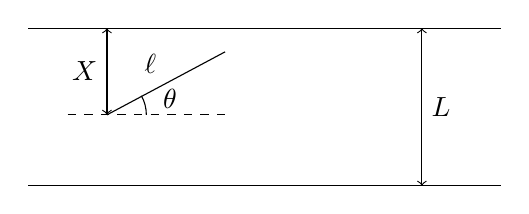
\begin{tikzpicture}
      \draw (-3, -1) -- (3, -1);
      \draw (-3, 1) -- (3, 1);
      \draw (-2, -0.1) -- (-0.5, 0.7) node [anchor = south east, pos = 0.5] {$\ell$};
      \draw [->] (-2, -0.1) -- (-2, 1) node [left, pos = 0.5] {$X$};
      \draw [->] (-2, 1) -- (-2, -0.1);
      \draw [dashed] (-2.5, -0.1) -- (-0.5, -0.1);
      \draw (-1.5, -0.1) arc (0:29:0.5);
      \node at (-1.2, 0.1) {$\theta$};
      \draw [->] (2, -1) -- (2, 1) node [right, pos = 0.5] {$L$};
      \draw [->] (2, 1) -- (2, -1);
    \end{tikzpicture}
  \end{center}
  Suppose we toss the pin $n$ times, and it hits the line $N$ times. Then
  \[
    N\approx N(np, np(1 - p))
  \]
  by the Central limit theorem. Write $p'$ for the actual proportion observed. Then
  \begin{align*}
    \hat{\pi} &= \frac{2\ell}{(N/n) L} \\
    &= \frac{\pi 2\ell/(\pi L)}{p'}\\
    &= \frac{\pi p}{p + (p' - p)}\\
    &= \pi \left(1 - \frac{p' - p}{p} + \cdots \right)
  \end{align*}
  Hence
  \[
    \hat\pi - \pi \approx \frac{p - p'}{p}.
  \]
  We know
  \[
    p' \sim N\left(p, \frac{p(1 - p)}{n}\right).
  \]
  So we can find
  \[
    \hat \pi - \pi \sim N\left(0, \frac{\pi^2 p(1 - p)}{np^2}\right) = N\left(0, \frac{\pi^2(1 - p)}{np}\right)
  \]
  We want a small variance, and that occurs when $p$ is the largest. Since $p = 2\ell/\pi L$, this is maximized with $\ell = L$. In this case,
  \[
    p = \frac{2}{\pi},
  \]
  and
  \[
    \hat \pi - \pi \approx N\left(0, \frac{(\pi - 2)\pi^2}{2n}\right).
  \]
  If we want to estimate $\pi$ to 3 decimal places, then we need
  \[
    \P(|\hat \pi - \pi| \leq 0.001) \geq 0.95.
  \]
  This is true if and only if
  \[
    0.001\sqrt{\frac{2n}{(\pi - 2)(\pi^2)}} \geq \Phi^{-1}(0.975) = 1.96
  \]
  So $n\geq 2.16 \times 10^7$. So we can obtain $\pi$ to 3 decimal places just by throwing a stick 20 million times! Isn't that exciting?
\end{eg}

\ifx \nhtml \undefined
\begin{landscape}
\section{Summary of distributions}
\subsection{Discrete distributions}
\begin{center}
  \begin{tabular}{ccccc}
    \toprule
    \textbf{Distribution} & \textbf{PMF} & \textbf{Mean} & \textbf{Variance} & \textbf{PGF} \\
    \midrule
    Bernoulli & $p^k(1 - p)^{1 - k}$ & $p$ & $p(1 - p)$ & $q + pz$\\
    Binomial & $\displaystyle\binom{n}{k}p^k(1 - p)^{n - k}$ & $np$ & $np(1 - p)$ & $(q + pz)^n$\\
    Geometric & $(1 - p)^k p$ & $\displaystyle\frac{1 - p}{p}$ & $\displaystyle\frac{1 - p}{p^2}$ & $\displaystyle\frac{1 - p}{1 - pz}$\\
    Poisson & $\displaystyle\frac{\lambda^k}{k!}e^{-\lambda}$ & $\lambda$ & $\lambda$ & $e^{\lambda(z - 1)}$\\
    \bottomrule
  \end{tabular}
\end{center}
\subsection{Continuous distributions}
\begin{center}
  \begin{tabular}{cccccc}
    \toprule
    \textbf{Distribution} & \textbf{PDF} & \textbf{CDF} & \textbf{Mean} & \textbf{Variance} & \textbf{MGF} \\
    \midrule
    Uniform & $\displaystyle\frac{1}{b - a}$ & $\displaystyle\frac{x - a}{b - a}$ & $\displaystyle\frac{a + b}{2}$ & $\displaystyle \frac{1}{12}(b - a)^2$ & $\displaystyle\frac{e^{\theta b} - e^{\theta a}}{\theta (b - a)}$ \\
    Normal & $\displaystyle \frac{1}{\sqrt{2\pi}\sigma}\exp\left(-\frac{(x - \mu)^2}{2\sigma^2}\right)$ & / & $\mu$ & $\sigma^2$ & $e^{\theta\mu + \frac{1}{2}\theta^2\sigma^2}$\\
    Exponential & $\lambda e^{-\lambda x}$ & $1 - e^{-\lambda x}$ & $\displaystyle \frac{1}{\lambda}$ & $\displaystyle\frac{1}{\lambda^2}$ & $\displaystyle\frac{\lambda}{\lambda - \theta}$ \\
    Cauchy & $\displaystyle \frac{1}{\pi(1 + x^2)}$ & / & undefined & undefined & undefined\\
    Gamma & $\displaystyle \frac{\lambda^n x^{n - 1}e^{-\lambda x}}{(n - 1)!}$ & / & $\displaystyle\frac{n}{\lambda}$ & $\displaystyle \frac{n}{\lambda^2}$ & $\displaystyle\left(\frac{\lambda}{\lambda - \theta}\right)^n$ \\
    Multivariate normal & $\displaystyle \frac{1}{(2\pi)^{n/2}\sqrt{\det \Sigma}} \exp\left[-\frac{1}{2}(\mathbf{z} - \boldsymbol\mu)^T\Sigma^{-1}(\mathbf{z} - \boldsymbol\mu)\right]$ & / & $\boldsymbol\mu$ & $\Sigma$ & /\\
    \bottomrule
  \end{tabular}
\end{center}
\end{landscape}
\fi
\end{document}

